%%%%%%%%%%%%%%%%%%%%%%%%%%%%%%%%%%%%%%%%%%%%%%%%%%%%%%%%%%%%%%%%%%%%%%%%%%%%%
%%%
%%% File: thesis.tex, version 1.9, May 2016
%%%
%%% =============================================
%%% This file contains a template that can be used with the package
%%% cs.sty and LaTeX2e to produce a thesis that meets the requirements
%%% of the Computer Science Department from the Technical University of Cluj-Napoca
%%%%%%%%%%%%%%%%%%%%%%%%%%%%%%%%%%%%%%%%%%%%%%%%%%%%%%%%%%%%%%%%%%%%%%%%%%%%%

\documentclass[12pt,a4paper,twoside]{report}         
\usepackage{cs}              
\usepackage{times}
\usepackage{graphicx}
\usepackage{latexsym}
\usepackage{amsmath,amsbsy}
\usepackage{amssymb}
\usepackage[matrix,arrow]{xy}
\usepackage[T1]{fontenc}
\usepackage{ae,aecompl}
\usepackage{romanian} %definitii pentru diacritice; 
\usepackage{amstext}
\usepackage{graphics}
\usepackage[T1]{fontenc}
\usepackage{ae,aecompl}
%\usepackage{algorithm}
%\usepackage{algorithmic}
\usepackage{color}
\usepackage{color}
\usepackage{listings}
\usepackage{verbatim}
\usepackage{subcaption}

\usepackage{algorithm2e}


% \mastersthesis
\diplomathesis
% \leftchapter
\centerchapter
% \rightchapter
\singlespace
% \oneandhalfspace
% \doublespace

\renewcommand{\thesisauthor}{Nicoleta COROCEA}    %% Your name.
\renewcommand{\thesismonth}{Iunie}     %% Your month of graduation.
\renewcommand{\thesisyear}{2019}      %% Your year of graduation.
\renewcommand{\thesistitle}{EXPLAINABLE MACHINE LEARNING USING ONTOLOGIES } % Title
\renewcommand{\thesissupervisor}{Assoc.Prof.Dr.Eng. Adrian GROZA}
\newcommand{\department}{FACULTATEA DE AUTOMATIC'A 'SI CALCULATOARE\\
DEPARTAMENTUL CALCULATOARE}
\newcommand{\thesis}{LUCRARE DE LICEN'T'A}
\newcommand{\uline}[1]{\rule[0pt]{#1}{0.4pt}}
%\renewcommand{\thesisdedication}{P'arin'tilor mei}
\newcommand{\utcnlogo}{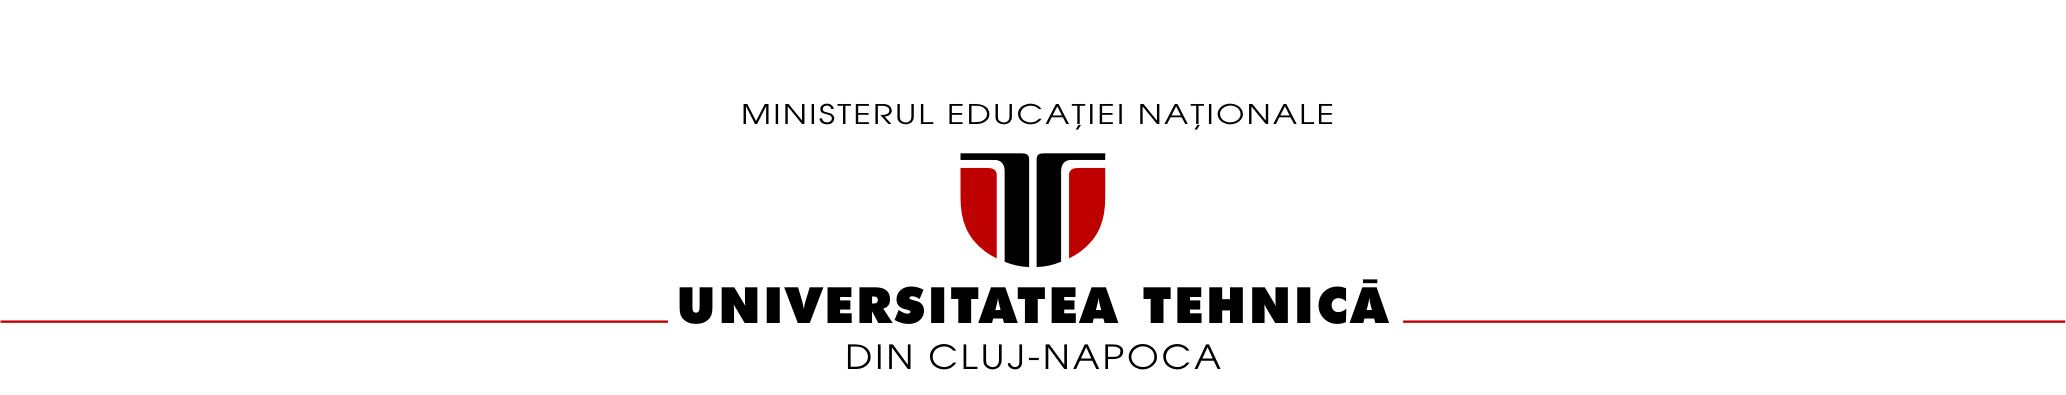
\includegraphics[width=15cm]{img/utcn.jpg}}
\newtheorem{example}{Exemplu}
\begin{document}

%\frontmatter
%\pagestyle{headings}

\newenvironment{definition}[1][Defini'tie.]{\begin{trivlist}
\item[\hskip \labelsep {\bfseries #1}]}{\end{trivlist}}



%\thesistitle                    %% Generate the title page.
%\authordeclarationpage                %% Generate the declaration page.


\begin{center}
%\includegraphics[width=15cm]{img/tucn.jpg}  
\utcnlogo

{\bf \department}

\vspace{4cm}

{\bf \thesistitle} %LICENSE THESIS TITLE}

\vspace{1.5cm}

\thesis

\vspace{6cm}

Absolvent: {\bf \thesisauthor} 

Conduc'ator 'stiin'tific: {\bf \thesissupervisor}

\vspace{3cm}
{\bf \thesisyear}
\end{center}

\thispagestyle{empty}
\newpage

\begin{center}
\utcnlogo

{\bf \department}
\end{center}
\vspace{0.5cm}

%\begin{small}
\begin{tabular}{p{7cm}p{8cm}}
 %\hspace{-1cm}& VIZAT,\\
 \hspace{-1cm}DECAN, & DIRECTOR DEPARTAMENT,\\
\hspace{-1cm}{\bf Prof. dr. ing. Liviu MICLEA} & {\bf Prof. dr. ing. Rodica POTOLEA}\\  
\end{tabular}
 
\vspace{2cm}

\begin{center}
Absolvent: {\bf \thesisauthor}

\vspace{1cm}

{\bf \thesistitle}
\end{center}

\vspace{1cm}

\begin{enumerate}
 \item {\bf Enun'tul temei:} {\it Scurt'a descriere a temei lucr'arii de licen't'a 'si datele ini'tiale}
\item {\bf Con'tinutul lucr'arii:} {\it (enumerarea p'ar'tilor componente) Exemplu: Pagina de prezentare, aprecierile coordonatorului de lucrare, titlul capitolului 1, titlul capitolului 2, titlul capitolului n, bibliografie, anexe.}
\item {\bf Locul document'arii:} {\it Exemplu}: Universitatea Tehnic'a din Cluj-Napoca, Departamentul Calculatoare
\item {\bf Consultan'ti:}
\item {\bf Data emiterii temei:} 1 Noiembrie 2018
\item {\bf Data pred'arii:} 8 iulie 2019 {\it (se va completa data pred'arii)}
  \end{enumerate}
\vspace{1.2cm}

\hspace{6cm} Absolvent: \uline{6cm} 

\vspace{0.5cm}
\hspace{6cm} Coordonator 'stiin'tific: \uline{5cm} 
%\end{small}

\thispagestyle{empty}

\newpage

\begin{center}
\utcnlogo

{\bf \department}
\end{center}

\vspace{0.5cm}

\begin{center}
{\bf
Declara'tie pe proprie r'aspundere privind\\ 
autenticitatea lucr'arii de licen't'a}
\end{center}
\vspace{1cm}



Subsemnatul(a) \\
\uline{14.8cm}, 
legitimat('a) cu \uline{4cm} seria \uline{3cm} nr. \uline{4cm}\\
CNP \uline{9cm}, autorul lucr'arii \uline{2.8cm}\\
\uline{16cm}\\
\uline{16cm}\\
elaborat'a 'in vederea sus'tinerii examenului de finalizare a studiilor de licen't'a la Facultatea de Automatic'a 'si Calculatoare, Specializarea \uline{7cm} din cadrul Universit'a'tii Tehnice din Cluj-Napoca, sesiunea \uline{4cm} a anului universitar \uline{3cm}, declar pe proprie r'aspundere, c'a aceast'a lucrare este rezultatul propriei activit'a'ti intelectuale, pe baza cercet'arilor mele 'si pe baza informa'tiilor ob'tinute din surse care au fost citate, 'in textul lucr'arii 'si 'in bibliografie.

Declar, c'a aceast'a lucrare nu con'tine por'tiuni plagiate, iar sursele bibliografice au fost folosite cu respectarea legisla'tiei rom\ia ne 'si a conven'tiilor interna'tionale privind drepturile de autor.

Declar, de asemenea, c'a aceast'a lucrare nu a mai fost prezentat'a 'in fa'ta unei alte comisii de examen de licen't'a.

'In cazul constat'arii ulterioare a unor declara'tii false, voi suporta sanc'tiunile administrative, respectiv, \emph{anularea examenului de licen't'a}.

\vspace{1.5cm}

Data \hspace{8cm} Nume, Prenume

\vspace{0.5cm}

\uline{3cm} \hspace{5cm} \uline{5cm}

\vspace{1cm}
\hspace{9.4cm}Semn'atura

\thispagestyle{empty}

\newpage

%\clearpage 
%\newpage

%\begin{comment}
{\color{red}{\bf De citit 'inainte} (aceast'a pagin'a se va elimina din versiunea final'a)}:
\begin{enumerate}
 \item Cele trei pagini anterioare (foaie de cap'at, foaie sumar, declara'tie) se vor lista pe foi separate (nu fa't'a-verso), fiind incluse 'in lucrarea listat'a. 
 Foaia de sumar (a doua) necesit'a semn'atura absolventului, respectiv a coordonatorului.
 Pe declara'tie se trece data c\ia nd se pred'a lucrarea la secretarii de comisie.
 \item Pe foaia de cap'at, se va trece corect titulatura cadrului didactic 'indrum'ator, 'in englez'a (consulta'ti pagina de unde a'ti desc'arcat acest document pentru lista cadrelor didactice cu titulaturile lor).
 \item Documentul curent {\bf nu} a fost creat 'in MS Office. E posibil sa fie mici diferen'te de formatare. 
\item Cuprinsul 'incepe pe pagina nou'a, impar'a (dac'a se face listare fa't'a-verso), prima pagin'a din capitolul Introducere tot a'sa, fiind numerotat'a cu 1. % Pentru actualizarea cuprinsului, click dreapta pe cuprins (zona cuprinsului va apare cu gri), Update field-$>$Update entire table.
\item Vizualiza'ti (recomandabil 'si 'in timpul edit'arii) acest document % după ce activaţi vizualizarea simbolurilor ascunse de formatare (apăsaţi simbolul  din Home/Paragraph).
\item Fiecare capitol 'incepe pe pagin'a nou'a. % datorită simbolului ascuns Section Break (Next Page) care este deja introdus la capitolul precedent. Dacă ştergeţi din greşeală simbolul, se reintroduce (Page Layout -> Breaks).
\item Folosi'ti stilurile predefinite (Headings, Figure, Table, Normal, etc.)
\item Marginile la pagini nu se modific'a.
\item Respecta'ti restul instruc'tiunilor din fiecare capitol.
\end{enumerate}
\thispagestyle{empty} 
%\end{comment}

\pagenumbering{roman}
\setcounter{page}{1}

\newpage

\tableofcontents

\newpage

%\listoftables
%\listoffigures

\pagenumbering{arabic}
\setcounter{page}{1}

%%%%%%%%%%%%%%%%%%%%%%%%%%%%%%%%%%%%%%%%%%%%%%%%%%%%%%%%%%%%%%%%%%%%%%%
\chapter{Introducere - Contextul proiectului}
\pagestyle{headings}
\section{Descrierea problemei}
\section{Conturarea solu'tiei}

%%%%%%%%%%%%%%%%%%%%%%%%%%%%%%%%%%%%%%%%%%%%%%%%%%%%%%%%%%%%%%%%%%%%%%%%%
\chapter{Obiectivele Proiectului}

'In acest capitol se vor descrie obiectivele sistemului dezvoltat, c\ia t 'si pozi'tionarea solu'tiei alese. De asemenea, sunt prezentate 'si descrise pe scurt 'si cerin'tele sistemului.

\section{Pozi'tionarea sistemului}
\section{Descrierea obiectivelor}
\section{Cerin'tele sistemului}
\subsection{Cerin'te fun'tionale}

\begin{itemize}
    \item {\it Translatarea limbajului natural 'in SPARQL} - Sistemul trebuie s'a pun'a la dispozi'tie un mecanism de translatare a 'intreb'arilor din limbaj natural 'in limbaj de interogare SPARQL, precum 'si o modalitate de editare ulterioar'a a interog'arilor.
    \item {\it Interogarea\ ontologiei} -  Sistemul trebuie s'a permit'a interogarea ontologiei utiliz\ia nd limbajul de interogare SPARQL destinat ontologiilor 'si s'a ofere r'aspunsuri pe baza resurselor conceptualizate 'in baza de cuno'stin'te, utiliz\ia nd libr'aria Pellet 'si libr'aria RDFLib.
    \item {\it Permite\ vizualizarea\ elementelor\ ontologiei} - Sistemul trebuie s'a ofere capabilitatea de a expune, prin intermediul interfe'tei utilizator, a tuturor elementelor din care este constituit'a ontologia.
\end{itemize}
\subsection{Cerin'te nonfunc'tionale}
\begin{itemize}
    \item {\it Utilizabilitate} - Proiectarea sistemului 'si a interfe'tei utilizator se va face urm'arind simplitatea de utilizare. Clien'tii novici pot 'incepe utilizarea cu pu'tin instructaj asupra utiliz'arii aplica'tiei.
    \item {\it Toleran'ta\ la\ e'sec} - Sistemul este construit 'in a'sa fel 'inc\ia t, 'in cazul in care acesta e'sueaz'a 'in interpretarea intreb'arii sau pentru g'asirea unui r'aspuns, utilizatorul va fi rugat s'a repete 'intrebarea sub o alta forma sau s'a verifice interogarea.
    \item {\it Securitate} - Datele ontologiei pot fi vizualizate, fiind publice utilizatorilor, dar nu se va permite realizarea interog'arilor care pot modifica  sau altera starea acestora.
    \item Explicativ
\end{itemize}

%%%%%%%%%%%%%%%%%%%%%%%%%%%%%%%%%%%%%%%%%%%%%%%%%%%%%%%%%%%%%%%%%%%%%%%%
\chapter{Studiu Bibliografic}

\section{XAI}
\section{Sisteme 'intrebare - r'aspuns}
\section{Structurarea 'si interogarea cuno'stin'telor}
\section{Ontologii ale domeniului 'inv'a't'arii automate}

%%%%%%%%%%%%%%%%%%%%%%%%%%%%%%%%%%%%%%%%%%%%%%%%%%%%%%%%%%%%%%%%%%%%%%
\chapter{Analiz'a 'si Fundamentare Teoretic'a}
\label{ch:analysis}

\section{Fundamentare conceptual'a}
%%%%========================================
\subsection{Dezvoltarea 'si utilizarea ontologiilor}


O ontologie reprezint'a o specificarea  conceptualiz'arii, 'in domeniul 'imp'art'a'sirii cuno'stin'telor. Este o descriere a conceptelor 'si a rela'tiilor care pot exista 'intr-un domeniu. Termenul de $ontologie$ este 'imprumutat din filozofie unde se refer'a la {\it existen't'a}. 'Intr-adev'ar, ceea ce exist'a poate fi reprezentat: o mul'time de obiecte care apar'tin unor concepte (numite 'si concepte) diferite 'si au 'intre ele roluri(numite 'si propriet'a'ti) care le leag'a.

Motiva'tia dezvolt'arii unei ontologii este descris'a de Deborah L. McGuinness et al. 'in ghidul \cite{protege_ontology}, propus de universitatea Standford. Principalul motiv al dezvolt'arii unei ontologiii este distribuirea unei structuri a informa'tiei 'intre oamneni sau agen'ti software. Astfel, agen'tii ar putea s'a r'spund'a 'intreb'arilor oamenilor, am\ia ndou'a p'ar'tile cunosc'and aceea'si schem'a. Un alt motiv al dezvolt'arii ontologiilor amintit 'in acest document este reutilizarea cuno'stin'telor. Prin acesta, se 'in'telege c'a mai mul'ti agen'ti pot refolosi domenii complexe, f'ar'a a fi necesar'a redefinirea acestora. 

O ontologie este format'a din $ABox$, $TBox$  'si $RBox$. $TBox$ reprezint'a un set de axiome terminologice, cum ar fi indivizii. $ABox$ reprezint'a un set de axiome sub form'a de aser'tii, cum ar fi clasele. $RBox$ con'tine rolurile care leag'a 'intre ele elementele din $TBox$. 

Un exemplu de ontologie este figura ~\ref{fig:onto_ex}. Clasele sunt $Audience$, $Artist$ 'si $Song$. $Spectator$, $Pianist$, $Piano\ Song$  sunt instan'te ale acestor clase. Pianistul c\ia nt'a un c\ia ntec la pian, iar spectatorul 'il ascult'a. Spectatorul 'si pianistul se pot vedea reciproc.

\begin{figure}
    \centering
    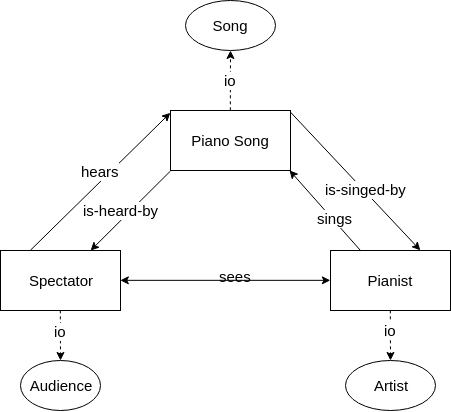
\includegraphics[width = 0.6\linewidth]{img/onto_example.png}
        \caption{Exemplu de ontologie}
    \label{fig:onto_ex}
\end{figure}

'In \cite{Press2014AdrianApproach}, Adrian Groza identific'a practicile rele care trebuie evitate 'in design-ul ontologiilor. O prim'a practic'a defectuoas'a este utilizarea rela'tiei $is$ deoarece se poate produce confuzie 'intre rela'tia de apartenen't'a 'si rela'tia ce define'ste o subclas'a. Trebuie evitate rela'tiile inverse care nu sunt declarate 'si clasele care nu au indivizi. Clasele care de'tin un num'ar mult prea mare de subclase trebuie re-evaluate deoarece poate s'a se realizeze o noua ierarhie, mai specific'a. Indivizii nu trebuie trata'ti ca 'si clasele: unele elemente, cum ar fi un nume de ora's, trebuie tratate ca indivizi.

Diana Kalibatiene \cite{owl_languages} face o clasificare a limbajelor de implementare a ontologiilor. Sunt identificate dou'a categorii de limbaje pentru ontologii, 'si anume: limbaje tradi'tionale 'si limbaje bazate pe Web. 

Din prima categorie, a limbajelor tradi'tionale, face parte KIF\footnote{http://www-ksl.stanford.edu/knowledge-sharing/kif/}. Acesta este un limbaj cu semantic'a declarativ'a, este cuprinz'ator din punct de vedere logic. Pune la dispozi'tie defini'tii pentru obiecte, func'tii 'si rela'tii.

Din categoria a doua, a limbajelor destinate web-ului semantic, fac parte urm'atoarele:

\begin{itemize}
    \item OWL ({\it Web Ontology Language}) - include exprimarea conjunc'tiilor, a disjunc'tiilor, a variabileleor cuatificate universal. Acestea pot fi folosite pentru a ob'tine cunos'tin'te noi prin realizarea inferen'telor logice. Con'tine $OWL\ Lite$, $OWL\ DL$ 'si $OWL\ Full$ ca sublimbaje.
    \item RDF({\it Resource\ Description\ Language}). Este scris 'in XML 'si este destinat 'in'telegerii de c'atre calculatoare, nu de c'atre oameni. Resursele identificate sunt exprimate sub form'a de triple: subiect, predicat 'si un obiect. 
    \item OIL ({\it Ontology Interchange Language}) este bazat pe RDFS 'si DL. A fost creat pentru a fi 'in'teles 'in mod intuitiv de utilizatori. 
    \item DARPA Agent Markup Language (DAML) - const'a 'in dou'a p'ar'ti: limbajul ontologiei  'si un limbaj pentru exprimarea constr\ia ngerilor 'si pentru ad'augarea regulilor de inferen't'a.
\end{itemize}

'Intr-o ierarhie a limbajelor de dezvoltare a ontologiilor, OWL se afl'a mai sus ca RDF, reprezent\ia nd un nivel de expresivitate mai 'inalt ca RDF. OWL adaug'a semantic'a schemei 'si permite specificarea mai multor detalii despre propriet'a'ti 'si clase. Av\ia nd urm'atoarele axiome exprimate 'in DL:

\begin{tabular}{ll}
          &  {\it (A, B):\ ancestorOf}\\
          &  {\it (B, C):\ ancestorOf}\\
\end{tabular}

OWL, spre deosebire de RDF, va implica 'si axioma {\it (A, C): ancestorOf}. 

Pentru a genera concluzii din cuno'stin'tele valabile folosind tehncii logice precum deduc'tia, se folose'ste un reasoner. Pellet, Racer, HermiT sunt unele dintre sistemele disponibile pentru reasoning. Acestea sunt detaliate 'in sec'tiunea ~\ref{sec:pellet}.

Pentru ob'tinerea informa'tiilor din ontologie, este necesar'a utilizarea limbajelor de interogare specifice. Pentru interogarea ontologiilor dezvoltate 'in OWL, sunt cunoscute limbajele de interogare SQWRL 'si SPARQL. Printre limbajele de interogare utilizate pentru ontologiile dezvoltate cu RDF se num'ar'a: RQL, SeRQL 'si RDQL.



%%%%%%%%=================================
\subsection{Procesarea limbajului natural}

Limbajul natural este complex 'si divers, av\ia nd particularit'a'ti care difer'a de la limb'a la alta, de la o regiune la alt'a regiune. Procesarea limbajului natural 'incearc'a s'a g'aseasc'a o solu'tie pentru a ajuta sistemele computerizate s'a 'inteleag'a limbajul scris sau vorbit al unui om. 

'In procesarea limbajului natural, exist'a dou'a tehnici utilizate: {\it analiza\ sintactic'a} 'si {\it analiza\ semantic'a}.

Analiza sintactic'a se refer'a la modul 'in care sunt aranjate cuvintele 'intr-o propozi'tie astfel 'inc'at sa aib'a semns din punct de vedere gramatic. Aceasta este utilizat'a in procesarea limbajului natural pentru a studia 'in ce mod se aliniaz'a acesta cu regulile gramaticale. 'In acest context, sunt utiliza'ti algoritmi pentru a aplica regulile gramaicale unor propozi'tii 'in vederea deriv'arii unui 'in'teles din acestea. C'ateva procedee pentru analiza sintactic'a sunt: lemmatizarea, segmentarea, etichetarea p'ar'tilor vorbirii, parsarea 'si stemming-ul.

{\it Lemmatizarea} implic'a reducerea unui cuv\ia nt la forma de baz'a, din dic'tionar, a acestuia: 

\begin{center}
{\it Lemma("is") = be}
\end{center}

{\it Segmentarea} presupune divizarea textului 'in unit'a'ti precum cuvinte sau propozi'tii. 

{\it Etichetarea p'ar'tilor vorbirii} const'a 'in identificarea p'ar'tilor sintactice ale vorbirii pentru fiecare cuv\ia nt al propozi'tiei. De exemplu, pentru propozi'tia {\it Alice\ has\ a\ nice\ umbrella}, felul 'in care p'ar'tile vorbirii sunt etichetate pot fi observate 'in tabelul ~\ref{table:pos_Tag}.


\begin{table}
\caption{Etichetarea p'ar'tilor vorbirii}
\centering                          % tabel centrat 
\begin{tabular}{|c|c|c|}          % 4 coloane centrate 
\hline\hline                        % linie orizontala dubla
Cuv\i ant& POS & Denumire\\ [0.5ex]   % inserare tabel
%heading
\hline                              % linie orizontal simpla
Alice & NNP & substantiv propriu \\[1ex]    
has & VBZ & verb la persoana a 3-a \\[1ex]% [1ex] 
a & DT & determinant\\[1ex]
nice & JJ & adjectiv\\[1ex]
umbrella & NN & substantiv\\[1ex]
\hline                              
\end{tabular}
\label{table:pos_Tag} 
\end{table}


\begin{figure}
    \centering
    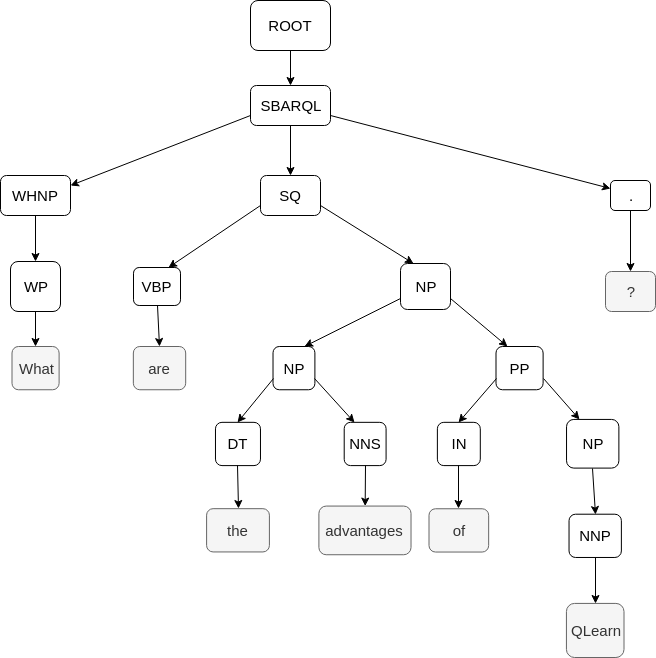
\includegraphics[width = 0.4\linewidth]{img/alice_parse.png}
        \caption{Exemplu de arbore sintactic}
    \label{fig:alice_parse}
\end{figure}

$Parsarea$ reprezint'a analiza automat'a a propozi'tiilor, 'tin\ia nd cont de strucura lor gramatic'a. Se atribuie etichete cu p'ar'ti de vorbire 'si se structureaz'a, 'in general, sub form'a de arbore sintactic. 'In figura ~\ref{fig:alice_parse} poate fi observat un exemplu al arborelui sintactic pentru propozi'tia $Alice\ has\ a\ nice\ umbrella.$


$Stemming-ul$ const'a 'in reducerea cuvintelor la forma dat'a de r'ad'acina lor. Aceast'a form'a nu trebuie s'a reprezinte un cuv\ia nt valid.

Analiza semantic'a presupune extragerea 'in'telesului din text. Analiza semantic'a a textului cuprinde determinarea p'ar'tilor de text 'si asocierea unei categorii acestora, oferirea sensului unui cuv\ia nt pe baza contextului, utilizarea bazelor de date pentru a ob'tine rela'tii semantice 'si pentru convertirea 'in limbaj natural a acestora.


Procesarea limbajului natural sus'tine interac'tiunile 'intre om 'si sistemele informatice. Un avantaj al utiliz'arii limbajului natural pentru exprimarea cerin'telor este acela c'a utilizatorii nu sunt nevoi'ti s'a se adapteze unui anumit mod de utilizare sau limbaj al sistemului.

%%%%%%%================================
\subsection{HTTP}
HTTP ({\it HyperText\ Transfer\ Protocol}) este un protocol an nivelului aplica'tie destinat transferului de informa'tii pe internet.
Acesta utilizeaza URI ({\it Uniform\ Resource\ Indentifier}) pentru identificarea resurselor 'si pentru stabilirea unei conexiuni cu acestea. HTTP este bazat pe o arhitectura client-server 'si interschimba informa'tii de-a lungul uncei conexiunii sigure TCP/IP.

Informa'tiile interschimbate au denumirea de mesaje 'si pot fi request-uri sau r'aspunsuri. Un request este f'acut de un client c'atre server pentru a ob'tine informa'tii, iar r'aspunsul este un mesaj trimis de la server c'atre client ca urmare a request-ului. 

Un mesaj este format din antet 'si corp. 'In antetul mesajului sunt puse la dispozi'tie informa'tii despre request sau r'aspuns, sau despre datele con'tinute de corp. Antetele pot fi generale, pentru request-uri, pentru r'aspunsuri sau de tip entitate. Corpul mesajului con'tine datele transmise odat'a cu request-ul sau r'aspunsul 'si poate fi op'tional 'intr-un mesaj HTTP. 

Cele mai importante metode HTTP pentru request sunt $GET$, $POST$, $PUT$, $DELETE$.
 $GET$ este utilizat'a pentru a ob'tine informa'tii, acesta neav\ia nd niciun efect colateral asupra datelor.
 $POST$ este folosit pentru a trimite date c'atre server. Datele sunt con'tinute de corpul request-ului.
 Pentru a 'inlocui anumite date pe server se folose'ste $PUT$. 'In acest caz, resursele sunt identificate printr-un URI. $DELETE$ este utilizat pentru a 'sterge datele identificate de URI de pe server.
La acestea se mai adaug'a 'si altele: $HEAD$, $CONNECT$, $OPTIONS$, $TRACE$.

Ca r'aspuns, pe l\ia nga resursele identificate, un mesaj HTTP mai con'tine si codul de status care anun'ta cum s-a efectuat request-ul. Un cod $1xx$ este un cod care anun't'a c'a request-ul a fost primit 'si procesarea datelor continu'a. Codul $2xx$ anun't'a succesul request-ului. 'In cazul 'in care este necesar s'a se fac'a o alt'a ac'tiune ce cons't'a 'intr-o redirec'tionare pentru a se duce la cap'at request-ul, se va primi un cod de tipul $3xx$. Eroarea unui client, cum ar fi sintaxa incorect'a, se rezum'a la codul de eroare din seria $4xx$. O eroare de server, 'in care acesta nu a reu'sit s'a 'indeplineasc'a cerin'ta datorit'a unor probleme interne chiar dac'a request-ul este valid, este semnalat'a prin codurile $5xx$

HTTP reprezint'a un protocol de comunicare de 'incredere utilizat pentru a transmite date peste protocolul TCP/IP. O extensie a HTTP este HTTPS care reprezint'a o versiune sigur'a, 'in care datele transmise sunt criptate.


\subsection{Inteligen'ta artificial'a explicativ'a}

XAI ($Explainable\ Artificial\ Intelligence$) reprezint'a o tehnic'a prin care deciziile sau comportamnetul unui agent inteligent pot fi u'sor de 'inteles de oameni. A ap'arut ca necesitate 'impotriva sistemelor $black\ box$ care cauzeaz'a scepticism 'si ne'incredere 'in r\ia ndul utilizatorilor.

Potrivit DARPA \cite{darpaXAI}, un agent inteligent ar trebui s'a raspund'a la 'intreb'ari precum 
"{\it De\ ce\ ai\ f'acut\ asta?}", 
"{\it C\ia nd\ reu'se'sti?}", 
"{\it C\ia nd e'suezi?}", 
"{\it C\ia nd pot avea 'incredere 'in tine?}", 
"{\it Cum\ corectez o eroare?}.". Programul $XAI$ dore'ste s'a creeze tehnici 'in special pentru machine-learning pentru a produce mai multe modele care pot fi explicate, p'astr\ia nd o bun'a performan't'a. Un alt obiectiv al acestui program este de a permite utilizatorilor s'a 'inteleag'a 'si s'a aib'a 'incredere 'in agen'tii inteligen'ti.

Explainable AI este esen'tial pentru a stabili 'increderea 'si a expune prin transparen'ta procesele care au loc pentru a genera un r'aspuns. Prin acesta, se poate garanta corectitudinea, iar utilizatorii pot 'intelege un output 'in func'tie de inputul utilizat.

\section{Unelte folosite}
\subsection{Angular}

Angular\footnote{Angular website https://angular.io/} este o unealt'a pentru construirea interfe'telor utilizator dinamice. Este u'sor de controlat 'si propune reutilizarea codului. Interfe'tele sunt construite pe baza HTML 'si TypeScript. 


\begin{figure}
    \centering
    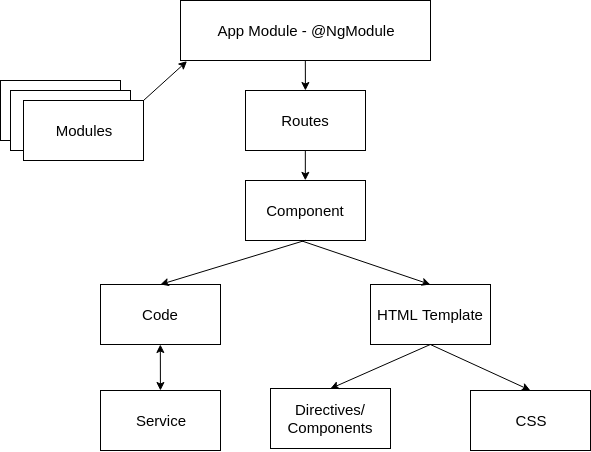
\includegraphics[width = 0.6\linewidth]{img/angular_schema.png}
        \caption{Arhitectura unei aplica'tii Angular}
    \label{fig:ang}
\end{figure}


O vedere de ansamblu a arhitecurii este prezentat'a 'in figura ~\ref{fig:ang} 'si este detaliat'a pe pagina oficial'a \cite{AngularCite}. Un $NgModule$ este cel mai de baz'a bloc al unei aplica'tii Angular, aceasta fiind definit''a de un set format din mai multe $NgModule$.

Modulele sunt un context de compilare, func'tionalit'a'ti de baz'a, pentru componente. Pentru a forma unit'a'ti func'tionale, componentele sunt asociate cu codul corespunz'ator (servicii).

Prin rutare, se pot defini c'ai de navigare prin diferite st'ari ale aplica'tiei sau view-uri. 'In loc de a mapa c'aile URL spre pagini, un $Router$ le va mapa spre view-uri. Pentru a defini noi reguli de navigare, se asociaz'a cai de navigare componentelor. Se poate utiliza logic'a 'in program pentru a restric'tiona sau a alege ce view-uri vor fi afis'ate.

Componentele sunt structuri importante care definesc o clas'a destinat'a logicii 'si datelor aplica'tiei. O component'a este asociat'a unui template HTML care reprezint'a un view ce va fi afi'sat. Orice aplica'tie Angular con'tine cel pu'tin o component'a, aceasta fiind componenta r'ad'acin'a. Aceasta define'ste o ierarhie care con'tine toate celelalte componente.

Un template HTML este scheletul ce con'tine elementele grafice disponibile utilizatorului. Acesta poate s'a con'tina, pe l\ia nga cod HTML propriu-zis, 'si directive Angular sau alte componente refolosite. Template-ul HTML este stilizat cu ajutorul unui fi'sier CSS.

\subsection{Spring Boot}
Spring Boot\footnote{Spring Boot https://spring.io/projects/spring-boot} este un framework Java, open-source, utilizat pentru crearea de microservicii. Un microserviciu implic'a o arhitectur'a care permite developerilor s'a dezvolte servicii independent.

Cu ajutorul Spring Boot se poate realiza cu u'surin'ta inversiunea controlului prin injectarea dependen'telor, ceea ce duce la dezvolarea unei aplica'tii cu cuplare joas'a. Alte beneficii aduse de Spring Boot sunt u'surin'ta 'in managementul dependen'telor, auto configurarea, disponibilitatea unui container pentru servleturi inclus 'si utilizarea adnot'arilor.

Adnor'arile sunt unul din punctele forte ale framework-ului, acestea permit'and configurarea aplica'tiei cu u'surin't'a. Printre adnot'arile utilizate des se num'ar'a $@SpringBootApplication$ care se utilizeaz'a 'in clasa ce reprezint'a punctul de start al aplica'tiei Spring Boot. Conform documenta'tiei oficiale \cite{springBootCite}, $@ComponentScan$ este utilizat pentru a semnala aplica'tiei care pachete con'tin clase ce ar trebui manageriate de Spring. Aceste clase pot include adnot'arile: 

\begin{itemize}
    \item $@Component$ - este utilizat sa denote o clas'a ca component'a. Astfel de clase sunt considerate $bean-uri$ 'si vor fi introduse 'in contextul aplica'tiei.
    \item $@Repository$ - este o specializare a adnot'arii $@Component$, fiind specific'a nivelului de $DAO$ al aplica'tiei. Excep'tiile ce sunt aruncate din nivelul de DAO vor fi traduse 'in $DataAccessException$, din Spring.
    \item $@Service$ - este o specializare a adnot'arii $@Component$ 'si nu pune la dispozi'tie alt comportament suplimentar fa't'a de aceasta. Este folosit'a pentru a exprima inten'tia de a realiza o clas'a din nivelul de service.
    \item $@Controller$ marcheaz'a o clas'a ca controller Spring MVC, fiind 'si aceasta o specializare a adnot'ariii $@Component$.
    \item $@RestController$ - este la r'ad'acin'a o combina'tie 'intre $@Controller$ 'si $@ResponseBody$,  pentru a permite facilit'a'tile date de acestea dou'a.
\end{itemize}

Alte adnot'ari des utilizate sunt $@RequestBody$, $@ResponseBody$, $@RequestMapping$ 'si $@Autowired$ . $@RequestBody$ indic'a faptul c'a parametrul metodei trebuie s'a fie legat de corpul request-ului web. $@ResponseBody$ este utilizat'a pentru a lega valoarea de return a metodei de corpul r'aspunsului dat de request-ul web. $@RequestMapping$ este folosit'a pentru a mapa request-urile web pe metode 'in clasele controller. Aceasta poate fi folosit'a at'at la nivel de clas'a, c\ia t 'si de metod'a, dar se prefer'a ca la nivel de metod'a se se foloseasc'a $@GetMapping$, $@PostMapping$, $@PutMapping$ sau $@DeleteMapping$. Adnotarea $@Autowired$ este utilizat'a pentru a injecta un bean 'intr-un atribut al clasei.

Fa'ta de framework-ul Spring original\footnote{Framework-ul Spring https://spring.io/}, Spring Boot pune la dispozi'tie autoconfigurarea. Acest lucru u'sureaz'a procesul de dezvoltare al aplica'tiei, ajung'and mult mai repede la un sistem executabil. Cu ajutorul $SpringBoot$, aplica'tia nu mai necesit'a a fi configurat'a prin XML, aceasta fiind auto-configurat'a prin adnot'ari.

\subsection{SPARQL}

SPARQL este un limbaj orientat pe date, acesta execut\ia nd interog'ari pe datele de'tinute 'intr-un model. Acesta identific'a informa'tiile pe baza constr\ia ngerilor 'si o returneaz'a sub forma de graf RDF sau a unui set de leg'aturi variabil'a-r'aspuns.

Potrivit \cite{sparql_tutorial}, o interogare SPARQL este format'a din declara'tii de prefix, definirea setului de date, clauza rezultatului, modelul de interogare 'si modificatori ai interog'arii.

Utilizarea operatorului $FILTER$ reprezint'a o practic'a 'int\ia lnit'a 'in interog'arile SPARQl. Acesta permite restric'tionarea valorilor dintr-un r'aspuns. $FILTER$ are aceea'si func'tioalitate ca operatorul $LIKE$ din limbajul SQL. 

Un exemplu care utilizeaz'a ontologia $Friend\ of\ a\ Friend$\footnote{FOAF http://www.foaf-project.org/} 'si cuprinde $FILTER$ este relatat 'in exemplul ~\ref{ex:sparql_ex}.



\begin{example}[Interogare SPARQL]
\begin{lstlisting}[basicstyle=\footnotesize, numbers=left, firstnumber = 0]

PREFIX foaf:  <http://xmlns.com/foaf/0.1/>

SELECT ?email
WHERE {
    ?person foaf:mbox ?email .
    ?person foaf:name ?name.
    FILTER(?name = foaf:Mary).
} ORDER BY ASC(?email)
\end{lstlisting}
\label{ex:sparql_ex}
\end{example}

'In acest exemplu, linia (1) reprezint'a declara'tia de prefix a ontlogiei FOAF. Pe linia (3) este se afl'a clauza rezultatului, variabila rezultat pe care o dorim returnat'a este $?email$. Liniile (5)-(7) reprezint'a modelul de interogare: se interogheaz'a dup'a o persoan'a ($?person$) care are emailul ($foaf:mbox$) dat de variabila $?email$. Prin $FILTER$ se reduce mul'timea rezultatelor la acelea 'in care numele persoanei este $Mary$. Linia (8) prezint'a un modificator de interogare, astfel ca lista de email-uri rezultat'a s'a fie ordonat'a asccendent.

Cu ajutorul operatorului $FILTER$ se pot executa 'si opera'tii care implic'a operatorii logici $and$ 'si $or$. Pentru a exprima c'a numele este $Mary$ 'si emailul este $mary@mary.com$, se poate folosi construc'tia: 
\begin{center}
{\it FILTER(?name\ =\ foaf:Mary\ \&\&\ ?email\ =\ foaf:mary@mary.com)}
\end{center}

Dac'a dorim s'a c'aut'am o persoan'a care are numele $Mary$ sau $Alice$, constr\ia ngerea pentru $FILTER$ se rezum'a la:
\begin{center}
{\it FILTER(?name\ IN(foaf:Mary, foaf:Alice))}
\end{center} 

Pentru implementarea unei nega'tii, se utilizeaz'a operatorul $MINUS$, dar aceasta nu este unica variant'a. O interogare 'in care se cer persoanele care nu au numele $Mary$ este ~\ref{ex:ex_minus}.

\begin{example}[Interogare SPARQL care utilizeaz'a operatorul MINUS]
\begin{lstlisting}[basicstyle=\footnotesize, numbers=left, firstnumber = 0]

PREFIX foaf:  <http://xmlns.com/foaf/0.1/>

SELECT ?person
WHERE {
    ?person foaf:name ?name.
    MINUS( ?name = foaf:Mary).
} 
\end{lstlisting}
\label{ex:ex_minus}
\end{example}

'In exemplul men'tionat, se va construi mul'timea tuturor persoanelor $person$ cu numele $name$. Din aceas'ta mul'time se va sc'adea mul'timea celor care au numele $Mary$. Astfel rezult'a mul'timea persoanelor care nua u numele $Mary$. Diferen'ta mul'timilor implementat'a cu $MINUS$ conduce la o nega'tie.

'In plus fa't'a de aceste func'tionalit'a'ti descrise, limbajul SPARQL permite 'si inserarea utiliz\ia nd $INSERT$, updatarea utiliz\ia nd $UPDATE$ 'si 'stergerea datelor folosind $DELETE$.

Utilizarea limbajului de interogare SPARQL implic'a o serie de avantaje. SPARQL permite utilizatorilor s'a interoghezze date de tipul cheie-valoare, cum ar fi date RDF. SPARQL pune la dispozi'tie o serie de unelte pentru a combina r'aspunsurile mai multor scheme. Datorit'a faptului c'a ontologiile sunt puse la dispozi'tie extern, se pot utiliza prefixe f'ara a crea ambiguit'a'ti.

%%%%%%%=========================
\subsection{Protege}
Protege\footnote{Protege http://www.smi.stanford.edu/projects/protege/overview/index.html} este o platform'a disponibil'a pentru dezvoltarea aplica'tiilor bazate pe ontologii sau modele de domeniu. 

Editorul Protege-OWL\footnote{Protege OWL http://www.smi.stanford.edu/projects/protege/overview/protege-owl.html} este o extensie a originalului Protege. Acesta sus'tine dezoltarea 'in limbajul OWL. Acesta pune la dispozi'tie facilit'a'ti importante lucrului cu ontologii, cum ar fi: 'inc'arcarea 'si salvarea ontologiilor 'in diverse formate printre care 'si OWL, RDF, Turte, Manchester-OWL; editarea ierarhiei de clase 'si integrarea propriet'a'tilor; definirea sub forma de expresii OWL a caracteristicilor logice ale claselor; utilizarea reasonerelor 'si a limbajelor de interogare.

Interfa'ta utilizator grafica a editorului Protege-OWL permite pentru clase ad'augarea claselor echivalente, a subclaselor, crearea de instan'te 'si ad'augarea de clase disjuncte. 

Pentru un individ, Protege-OWL permite semnalarea faptului c'a acesta reprezint'a aceea'si instan't'a sau instan'te diferite cu un alt individ. 'In leg'atur'a cu un individ se pot ad'auga propriet'a'ti-obiect c'atre al'ti indivizi sau propriet'a'ti-dat'a c'atre valori.

Interogarea ontologiei dezvoltate se poate face cu ajutorul interog'arilor SPARQL sau DL 'si a regulilor SWRL sau SQRL. 'In timpul realiz'arii acestor interog'ari, pentru a ob'tine r'aspunsuri complete, este necesar ca un reasoner s'a fie activ. Utilizatorul poate face uz de urm'atoarele unelte de reasoning: HermiT, Pellet 'si Pellet (Incremental).

'In cadrul interfe'tei grafice, utilizatorul are posibilitatea de a vizualiza ontologia dezvoltat'a prin intermediul unor plugin-uri specifice: GraphViz\footnote{GraphViz https://www.graphviz.org/} 'si OntoGraph\footnote{OntooGraph https://github.com/NinePts/OntoGraph}.


RacerPro este o variant'a alternativ'a pentru Protege-OWL, dar aceast'a variant'a este pus'a la dispozi'tie sub form'a comercial'a. Test'and sistemul accesibil f'ar'a plat'a, am constatat c'a nu permite interog'ari SPARQL.



\subsection{Pellet}
\label{sec:pellet}

Pellet \cite{SirinPellet:Reasoner} este un reasoner pentru OWL-DL dezvoltat de Bijan Parsia et al. Este scris 'in Java, iar codul este open-source\footnote{Repository Pellet https://github.com/stardog-union/pellet} 'si de'tine exemple de utilizare. Ofer'a suport extins pentru $reasoning$ cu indivizi folosind Jena sau interfe'te OW:-API. Acesta verific'a 'si consistent'a unui document OWL, retun\ia nd un raspuns de $consistent$, $inconsistent$ sau $necunoscut$.

Pellet cuprinde setul standard de servicii de inferen'ta in logic'a descriptiv'a, 'si anume: verificarea consisten'tei, satisfiabilitatea conceptelor, clasificare, realizare:
\begin{itemize}
    \item $Verificarea$ {\it consisten'tei} se asigur'a c'a ontologia nu con'tine fapte contradictorii.
    \item $Satisfiabilitatea$ $conceptelor$ verific'a dac'a exist'a posibilitatea pentru o clas'a s'a aib'a instan'te.
    \item $Clasificarea$ va crea 'intreaga ierarhie de clase pri verificarea tuturor rela'tiilor 'intre acestea. Acest serviciu permite g'asirea unui r'aspuns la interog'arile care implic'a 'si subclasele unei clase.
    \item $Realizarea$ poate fi utiliat'a dup'a $clasificare$ pentru a g'asi tipul direct sau toate tipurile fiec'arui individ, acesta fiind inclus 'in arborele clasific'arii.
\end{itemize}
   

Pentru a da un r'aspuns interog'arilor booleene, Pellet va reduce problema la una de insatisifiabilitate. 'In cazul 'in care un set de r'aspunsuri trebuie returnat, se vor calcula mai 'int\ia i r'aspunsurile evidente care constau 'in instan'te, iar apoi se caut'a non-instan'tele, 'incheind cu verficarea consisten'tei. 

Libr'aria Pellet con'tine un modul {\it Query\ Engine} pentru ABox pentru a r'aspunde interog'arilor conjunctive. Un major avantaj al acestui modul este c'a suport'a interog'ari 'in limbaj SPARQL sau RDQL.


'In \cite{tableau_alg} se aminte'ste c'a algoritmul $Tableau$ st'a la baza reasonerului Pellet. Reasonerele dezvoltate pe baza algoritmului $tableau$ sunt dezvoltate pentru o logic'a multi mai expresiv'a. Astfel de reasonere 'incearc'a s'a construiasc'a un model consistent 'si satisfiabil utiliz'and reguli de completare,'incerc'and s'a extind'a modelul p\ia n'a satisface toate axiomele.
%  O alt'a categorie de reasonere, cele care folosesc reasoning determinat de consecin'te, sunt foarte bine optimizate pentru ontologiile OWL care con'tin logic'a Horn. Pentru ob'tinerea r'aspunsului, acestea aplic'a reguli de deducere pentru a infera  entailments (urm'arile) unor axiome din ontologie.

Conform \cite{SirinPellet:Reasoner} unde s-a realizat o compara'tie cu alte reasonere, Pellet func'tioneaz'a mai bine ca RacerPro, fiind testat pe 3 seturi de date pentru a ajunge la aceast'a concluzie. 'In compara'tie cu FaCT++ 'si cu RacerPro, Pellet nu este la fel de rapid 'in task-uri care implic'a reasonig pe TBox. 

Un avantaj major al libr'ariei Pellet 'in compara'tie cu RacerPro este acela c'a timpul de extragere al unui r'aspuns nu este influen'tat de dimensiunea r'aspunsului. 

HermiT este un alt reasoner pentru OWL 2 care suport'a interog'ari SPARQL. Comparativ cu acesta, Pellet a classificat mai multe ontologii comparativ cu HermiT. Datorit'a suportului extins 'si u'surin'tei de utilizare 'si integrare,  Pellet reprezint'a cea mai bun'a variant'a pentru realizarea extragerii r'aspunsurilor dintr-o ontologie personal'a. 


\subsection{RDFLib}

RDFLib\footnote{https://rdflib.readthedocs.io/en/stable/} este un package Python destinat proces'arii datelor 'in limbaj RDF, limbaj care reprezint'a datele sub form'a de graf. Reprezentarea datelor cu RDF este sub form'a de triple: subiect-predict-obiect. RDFLib are suport pentru interog'ari SPARQL 'si con'tine parsere 'si serializatoare pentru N-Triples, RDF/XML, N-Triples\footnote{https://www.w3.org/TR/n-triples/}, Turtle\footnote{https://www.w3.org/TR/turtle/}.

De mare interes este modulul $Graph$ al acestei libr'arii care pune la dispozi'tie reprezentarea triplelor RDF sub form'a de graf prin func'tia $parse()$. Pe aceste grafuri se pot realiza opera'tii cum ar fi: reuniune, diferen'ta 'sii intersec'tie. 'In plus fa'ta de aceste opera'tii, se pot face itera'tii pe graf.


RDFLib aduce cu sine o implementare a limbajelor SPARQL pentru interogare 'si update. Sunt puse dou'a func'tii, $query()$ 'si $update()$ la dispozi'tie pentru 'indeplinirea acestor avantaje. Func'tiile pentru interogare 'si update utilizeaz'a reprezentarea sub form'a de graf pentru a ob'tine r'aspunsuri. Aceste r'aspunsuri sunt sub forma de leg'aturi varibil'a-obiect.
\subsection{Quepy}

Quepy este un framework Python 2 destinat transform'arii 'intreb'arilor din limbaj natural 'in interog'ari care pot fi utilizate pentru baze de date sau ontologii. Acesta ofer'a suport petru limbajul de interogare SPARQL ($SPARQL\ Protocol\ and\ RDF\ Query\ Language$) 'si MQL ($Model\ Query\ Language$). 

Pentru o bun'a func'tionare a aplica'tiei, trebuie instalate 'in prealabil urm'atoarele libr'arii de care depinde Quepy:  $REfO$\footnote{REfO webpage https://pypi.org/project/REfO/}, $nltk$\footnote{nltk webpage http://www.nltk.org/}, $SPARQLWrapper$\footnote{SPARQLWrapper webpage https://pypi.org/project/SPARQLWrapper/} 'si, op'tional, $graphviz$\footnote{graphviz webpage http://www.graphviz.org/} pentru vizualizarea interog'arilor.
Conform, documenta'tiei acestui framework \cite{quepyCite}, trebuie parcur'si c\ia 'tiva pa'si pentru a realiza o aplica'tie Quepy. 

Libr'aria $REfO$ este utilizat'a pentru oferi suport expresiilor regulate pentru obiecte. Comparativ cu alte libr'arii destinate expresiilor regulate ce identific'a 'siruri de caractere, REfO este utilizat pentru a identifica secven'te arbitrare de obiecte. 

Libr'aria $nltk$ este o platform'a destinat'a aplica'tiilor Python pentru a interac'tiona cu limbajul natural. Pune la dispozi'tie resurse lexicale, dar 'si alte module pentru clasificarea, tokenizarea, etichetarea 'si parsarea propozi'tiilor 'in limbaj natural.

Libr'aria $SPARQLWrapper$ este un layer de interfa'tare pentru serviciile SPARQL. Aceasta este utilizat'a pentru transformarea 'si formatarea interog'arilor SPARQL intr-un format mai u'sor de 'in'teles.

Conform tutorialului oficial prezentat 'in documenta'tia Quepy, structura de baz'a a fiec'arui proiect Quepy con'tine urm'atoarele fi'siere: $projectname/parsing.py$, $projectname/dsl.py$, $projectname/settings.py$, $main.py$. 


'In $dsl.py$ se defineste limbajul specific al domeniului aplica'tiei, adic'a tabele, clase, rela'tii 'si caracteristici specifice unei baze de cuno'stin'te. Se pot folosi ca superclase urm'atoarele: $FixedDataRelation$ pentru a abstractiza o rela'tie c'atre o $Data$, $FixedRelation$ pentru a exprima rela'tia 'intre doua elemente, $FixedType$ pentru a abstractiza faptul c'a un element are un anumit tip, $HasKeyword$ pentru a decide care e cuv'antul cheie dup'a care vrem s'a selectam r'aspunsurile. 

'In exemplul ~\ref{ex:dsl}, folosind $FixedType$, $FixedRelation$ 'si un prefix $kb$ al unei ontologii despre ora'se, am definit doua clase 'in fi'sierul $dsl.py$: $IsPersonName$ 'si $HasAddress$.
\begin{example}[Clase din fisierul dsl.py]
\begin{lstlisting}[basicstyle=\footnotesize, language = Python]

class IsPersonName(FixedType):
    fixedtype = "kb:PersonName"
    
class HasAddress(FixedRelation):
    relation = "kb:has-address"
    reversed = True
\end{lstlisting}
\label{ex:dsl}
\end{example}

$IsPersonName$ define'ste o clas'a cu numele $PersonName$ din ontologia cu prefixul $kb$. $HasAddress$ define'ste o rela'tie fix'a $has-address$ a ontologiei date de prefixul $kb$, rolul variabile $reversed$ fiind de a folosi rela'tia invers'a.

Fi'sierul $parsing.py$ este folosit pentru definirea expresiilor regulate ce vor fi utilizate pentru a se potrivi cu 'intreb'arile 'in limbaj natural. Fiecare 'intrebare are asociat'a o clas'a 'in care expresiile regulate vor fi definite 'si interpretate apoi.

'In exemplul ~\ref{ex:parsing} am definit dou'a clase: $PersonName$ 'si $PersonHasAddress$. Acestea dou'a utilizeaz'a clasele $IsPersonName$ 'si $HasAddress$ din fi'sierul $dsl.py$.
\begin{example}[Clase din fisierul parsing.py]
\begin{lstlisting}[basicstyle=\footnotesize, language = Python]

class PersonName(Particle):
    regex = Pos("NN") | Pos("NNP")

    def interpret(self, match):
        name = match.words.tokens
        return IsPersonName() + HasKeyword(name)
    
class PersonHasAddress(QuestionTemplate):
    optional_opening = Question((Pos("WP") | Pos("WDT")) + Lemma("be") +
                    Pos("DT"))
    regex = optional_opening + Lemma("address") + \
             Pos("IN") + PersonName() + Question(Pos("."))

    def interpret(self, match):
        person = HasAddress(match.personname)
        return person, "enum"

\end{lstlisting}
\label{ex:parsing}
\end{example}

$PersonHasAddress$ define'ste expresia regulat'a pentru 'intrebarea:

\begin{tabular}{ll}
 & $What\ is\ the\ address\ of\ Maria?$
\end{tabular}


$Maria$ se potrive'ste cu expresia regulat'a definit'a de $PersonName$. Rezultatele selectate de interogare trebuie s'a fie nume de persoan'a 'si s'a aib'a cuv\ia ntul cheie $Maria$. Conform func'tiei $interpret$ din $PersonHasAddress$, rezultatele care pot fi date de interogare trebuie s'a aib'a o rela'tie invers'a de $has-address$ c'atre o persoan'a cu numele $Maria$.

'In continuare voi prezenta algoritmul ~\ref{alg:quepy} care reprezint'a fluxul de procesare al unei 'intreb'ari 'in cadrul aplica'tiei Quepy pentru a fi transformat'a 'in limbaj de interogare SPARQL.

  
\begin{algorithm}
\caption{Fluxul de procesare al unei 'intreb'ari folosind Quepy}
\label{alg:quepy}
 \KwData{Query $q$ in natural language}
 
 \KwResult{SPARQL query}
 
 $\mathcal{R} \leftarrow extractRules(\mathcal{Q})$\;
 
 $W_q \leftarrow tokenize(q)$\;
 
 $q_{SPARQL} = "\ "$\;

\ForEach {$r \in \mathcal{R}$}
{\If{$match(r, \mathcal{W}_q)$}{ 
\State $className = provenanceClass(r)$\; 
\State $graph[srcNode, (property, destNode)] = className.interpret(r, \mathcal{W}_q)$\;
\State $q_{SPARQL} = graphToSparql(graph)$
}        
%\EndIf
\textbf{return} $q_{SPARQL}$
}
\end{algorithm}


Inputul algoritmului este o 'intreare 'in limbaj natural, $q$. Primul pas const'a 'in extragerea tuturor regulilor definite 'in aplica'tie. Apoi, 'intrebarea utilizatorului este 'imp'ar'tit'a 'in tokeni, 'si i se atribuie etichete care identific'a ce parte a vorbirii este (substantiv, verb, prepozi'tie etc.), ob'tin\ia nd $W_q$. Rezultatul $q_{SPARQL}$ este 'ini'tializat. Pentru fiecare regul'a definit'a 'in mul'timea de reguli se verific'a dac'a se potrive'ste cu $W_q$. 'In cazul 'in care se potrive'ste, se ob'tine clasa 'in care a fost definit'a regula 'si 'in func'tie de metoda de interpretare, se adaug'a un noduri 'in graf care con'tin o tripl'a surs'a - proprietate - destina'tie. Se returnez'a interogarea SPARQL dup'a ce graful a fost interpretat. 'In cazul 'in care nu a fost indentificat'a o regul'a potrivit'a, se returneaz'a o interogare goal'a.

Potrivit analizei f'acute de Stein Seibu \cite{SteinSaebuOptiqueNLQF:Technologies}, framework-ul Quepy nu este scalabil, datorit'a necesit'a'tii de a introduce expresiile regulate manual. Pe de alt'a parte, un sistem care utilizeaz'a Quepy este mult mai u'sor de realizat fa't'a de celelalte proiecte asem'an'atoare: SINA \cite{Shekarpour2015SINA:Data} 'si Pythia \cite{Unger2011Pythia:Web}. Un alt avantaj al framework-ului Quepy este acela c'a este open source.


%%%%%%%%%%%%%%%%%%%%%%%%%%%%%%%%%%%%%%%%%%%%%%%%%%%%%%%%%%%%%%%%%%%%%%%%
\chapter{Proiectare de Detaliu 'si Implementare}

\section{Arhitectura sistemului}

'In cadrul acestei sec'tiuni se prezint'a o scurt'a descriere a aplica'tiei, iar 'in sec'tiunile urm'atoare vor fi prezentate pe larg fiecare dintre componente. Agentul explicativ pune la dispozi'tie o interfa'ta pentru utilizator 'in care acesta poate introduce 'intrebari, respectiv poate afla rezultatul acestora 'si termeni cheie ai ontologiei. Serverul asigur'a translatarea 'in limbaj de interogare SPARQL a 'intrebarii ini'tiale, rularea interog'arii prin metoda aleas'a de client 'si afi'sarea r'aspunsurilor 'in zona destinata acestuia.

Arhitectura agentului explicativ pe domeniul machine-learning este structurat'a pe niveluri, 'in care fiecare modul este independent si constituie un nivel. Acest lucru permite ca unele func'tionalit'a'ti s'a fie solu'tionate printr-o aplica'tie Java, iar altele cu ajutorul scripturilor Python. Figura ~\ref{fig:arch} ilustreaz'a arhitectura general'a a sistemului 'si maniera 'in care cele patru module comunic'a 'intre ele. 'In cadrul acestor componente, modulul serverului pentru inferen't'a joac'a un rol major, dac'a nu principal, toate apelurile provenite de la interfa'ta utilizator fiind procesate de acesta. Func'tionarea corect'a a serverului este esen'tial'a 'in aceast'a aplica'tie, dar 'si translatorul Quepy 'si ontologia asigur'a comportamentul adecvat al sistemului.

Interac'tiunea utilizatorului cu interfa'ta const'a 'in introducerea unei intreb'ari 'in limbaj natural 'si ac'tionarea comenzii pentru transformarea in limbajul de interogare SPARQL. Apelul va fi tratat de serviciul de inferen't'a {\it Reasoning Service}, prezentat 'in Fig. ~\ref{fig:arch}, care va realiza transformarea cu ajutorul translatorului Quepy, denumit 'in figura citata {\it Quepy translator}. Interogarea SPARQL va fi afi'sat'a 'si clientul are posibilitatea de a o modifica sau de a o executa fie folosind libraria Pellet, fie cu script-ul care utilizeaz'a RDFLib. R'aspunsul va fi prezentat 'in aria destinat'a. Utilizatorul mai are la dispozi'tie 'si o pagin'a 'in care poate solicita detaliile ontologiei: listarea claselor, a indivizilor 'si a propriet'a'tilor care le leag'a.


\begin{figure}
    \centering
    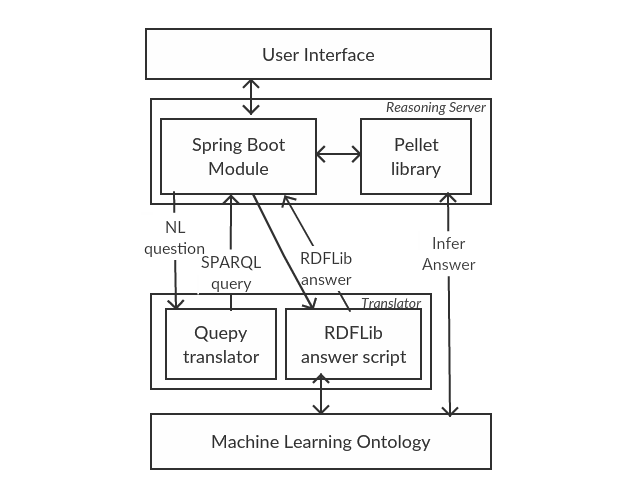
\includegraphics[width = 0.75\linewidth]{img/arhitectura-generala-black.png}
        \caption{Arhitectura sistemului}
    \label{fig:arch}
\end{figure}

Interfa'ta utilizator este construit'a simplu, 'in stil minimalist, astfel 'incat clientul s'a nu se piard'a 'in detalii. Este alc'atuit'a din dou'a pagini cu ajutorul c'arora utilizatorul poate chestiona datele 'in limbaj natural cu ajutorul librariei Pellet sau RDFLib sau poate ob'tine detalii despre ontologie. 

Serverul pentru inferen't'a, 'in imaginea mai sus men'tionat'a {\it Reasoning Service}, este consituit din libr'aria Pellet 'in care am integrat un modul Spring Boot pentru a pune la dispozi'tie sub form'a de endpoint-uri func'tionalit'a'tile necesare. Ca arhitectur'a, este format dintr-un nivel de control, un nivel de  servicii pentru ob'tinerea informa'tiilor de la libr'aria Pellet si de la modulul Python care utilizeaz'a RDFLib, 'si un nivel inferior pe care se afl'a libr'aria pentru inferen't'a.

Pe cel de-al treilea nivel al arhitecturii generale este pozi'tionat modulul Python denumit {\it Translator}. Acesta are doua func'tionalit'a'ti, o func'tionalitate pentru translatarea 'intreb'arilor din limbaj natural 'in SPARQL 'si una pentru interogarea ontologiei folosind libr'aria RDFLib. Translatorul Quepy este generat automat cu ajutorul framework-ului Quepy 'si con'tine clasele standard pentru parsare, pentru 'in'telegerea limbajului specific al domeniului 'si pentru ini'tializarea aplica'tiei. La acestea, se adaug'a un script pentru ob'tinerea unui r'aspuns cu ajutorul libr'ariei RDFLib.

Nivelul inferior const'a 'in ontologie, reprezent'and componenta care asigur'a persisten'ta datelor referitoare la machine learning. Indivizii acesteia sunt structura'ti 'in clase si subclase, depinz\ia nd unul de altul prin propriet'a'ti. O detaliere a arhitecturii ontologiei, c\ia t 'si a func'tionalita'tii 'si implement'arii fiec'arei componente mai sus amintite, va fi prezentat'a 'in cardul acestui capitol, 'in sec'tiunile care urmeaz'a. 

'In Figura ~\ref{fig:arch_det} se prezint'a modulele principale ale sistemului, 'impreuna cu modul detaliat de comunicare al acestora. Fluxul de informa'tii porne'ste de la utilizator 'si str'abate serverul pentru inferen't'a, {\it Reasoning Server}. 'In situa'tia 'in care s-a f'acut un apel pentru translatarea unei 'intreb'ari din limbaj natural 'in SPARQL sau pentru ob'tinerea r'aspunsului prin RDFLib, este utilizat 'si modulul {\it Translator}, 'in fun'tie de cerin'te. 

\begin{figure}
    \centering
    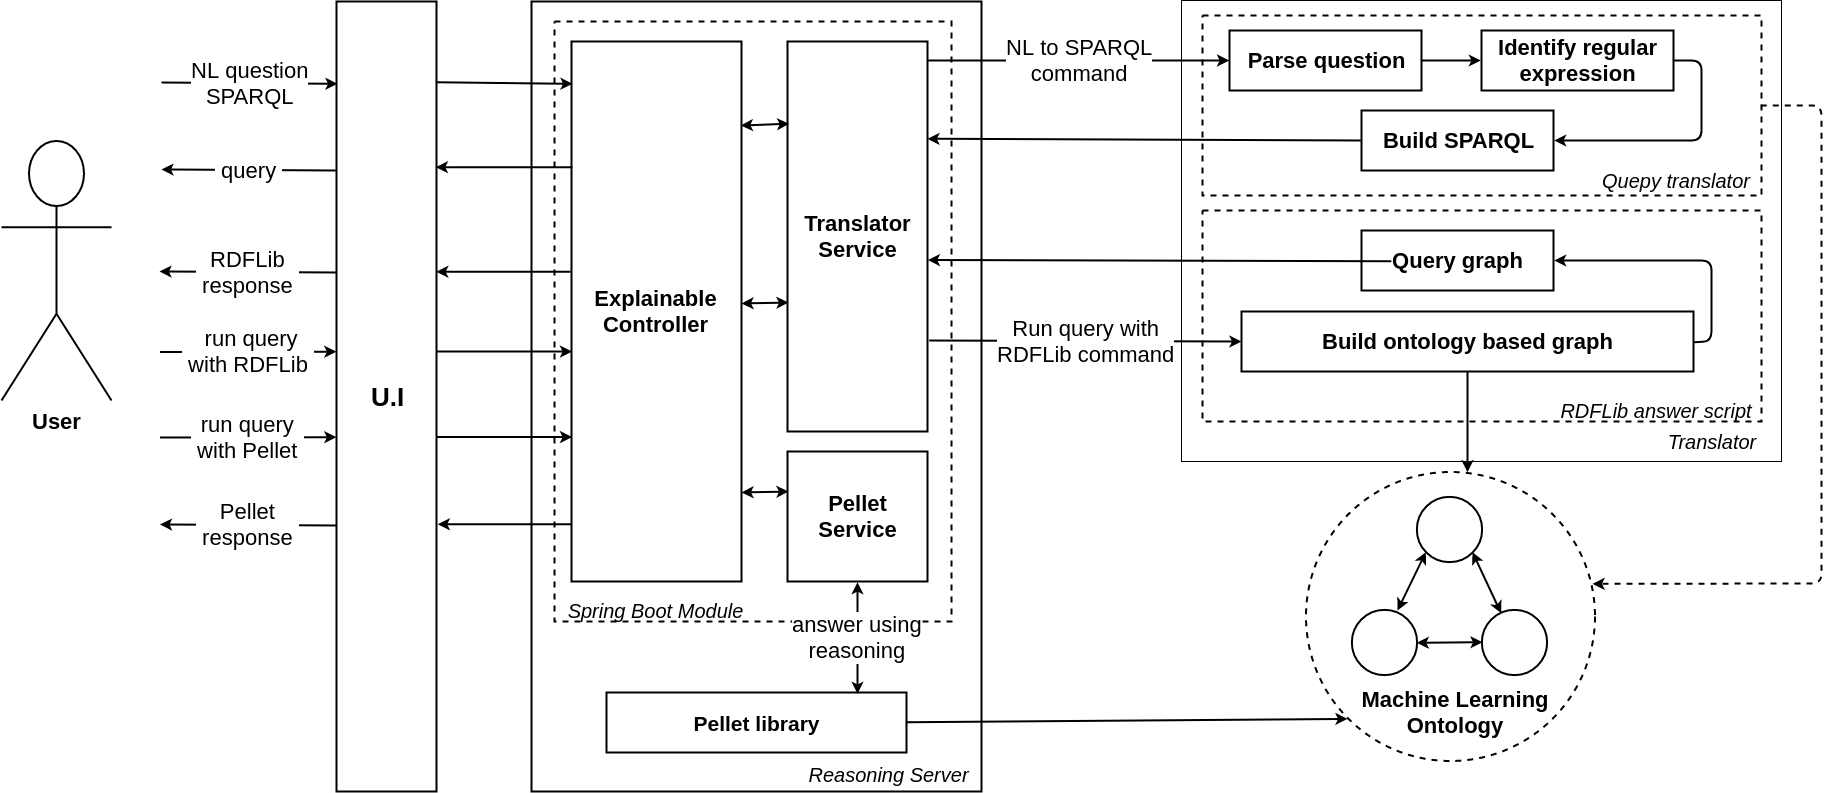
\includegraphics[width = 0.9\linewidth]{img/architecture_details.png}
        \caption{Elemente de comunicare 'in arhitectur'a}
    \label{fig:arch_det}
\end{figure}

Imaginea mai sus amintit'a pune 'in valoare trei situa'tii principale, care sunt folosite 'in mod global: translatarea unei 'intrebari 'in SPARQL cu ajutorul libr'ariei Quepy, interogarea r'aspunsului prin Pellet sau prin RDFLib. 'In toate aceste cazuri, se utilizeaz'a ontologia 'incarcat'a in memoria aplica'tiei sau se face uz de abstractizarea acesteia 'in cod, pentru modulul translatorului Quepy.

Primul pas al utilizatorului este de a insera 'intrebarea si de a activa apelul translat'arii acesteia. Serverul constituit din modulul Spring Boot va intercepta cerint'a 'in {\it Explainable Controller} 'si o va trece mai departe la serviciul dedicat, {\it Translator Service}. Acesta din urm'a execut'a comanda de rulare a modulului {\it Quepy translator}. Translatorul parseaz'a 'intrebarea, identific'a expresia regulat'a cu care se potrive'ste 'si contruie'ste interogarea SPARQL dintr-un graf generat de acest proces, apoi pune la dispozi'tie r'aspunsul pentru a fi preluat de {\it Reasoning Server}. Ca r'aspuns al apelului f'acut de utilizator, serverul va returna interogarea, iar aceasta va fi afi'sat'a 'in interfa'ta utilizator.

De'si primul pas poate fi omis 'si clientul poate s'a introduc'a manual interogarea pe care o dore'ste, rularea interog'arii aferente 'intreb'arii utilizatorului constituie al doilea pas logic 'in execu'tia cerin'tei. Utilizatorul activeaz'a comanda pentru rulare cu Pellet sau cu RDFLib din interfa'ta utilizator. 'In ambele cazuri, 'si atunci c'and dore'ste aflarea r'aspunsului prin inferen'ta sau prin extragere din graf, apelul va fi recep'tionat de controller. 

Dac'a ne afl'am 'in situa'tia 'in care se dore'ste aflarea r'aspunsului prin Pellet, controllerul  va 'inainta cererea la {\it Pellet Service}. Acesta o va solu'tiona cu ajutorul libr'ariei Pellet care de'tine modelul ontologiei 'in memorie 'si va extrage r'aspunsul prin reasoning. Astfel, 'si solu'tiile mai pu'tin evidente vor fi incluse 'in r'aspuns. R'aspusul este formatat de c'atre {\it Pellet Service} 'in format JSON pentru o lizibilitate crescut'a.

Solu'tionarea r'aspunsului prin graful RDFLib const'a in 'inaintarea apelului c'atre script-ul de ob'tinere a r'aspunsului bazat pe RDFLib, implementat 'in {\it Translator}. Pentru aflarea r'aspunsului, aceasta func'tie va citi ontologia sub form'a de graf RDF de la locatia precizat'a. Acest model RDF al ontologiei va fi interogat cu ajutorul query-ului transmis ca parametru 'si va returna un JSON cu rezultatele. Serviciul responsabil cu preluarea rezultatului este {\it Translator Service}. Acesta va returna controllerului rezultatul, care mai departe le va transmite interfe'tei utilizator, unde vor fi afi'sate.

Aplica'tia prezentat'a are o arhitectur'a structurat'a pe niveluri, oferind independe't'a 'intre module. Acest fapt aduce cu sine avantaje cum ar fi: func'tionarea aplica'tiei pe baza interogarilor directe 'in SPARQL 'in cazul 'in care modulul {\it Translator} nu func'tioneaz'a; 'inlocuirea ontologiei cu alta dintr-un domeniu diferit; asignarea atribu'tiilor clare 'si separate modulelor. 




\section{Modulul interfe'tei utilizator}

O necesitate a acestei aplica'tii, datorit'a nevoii interac'tiunii unor utilizatori cu aceasta, a fos tinterfa'ta utilizator. Aceasta a fost implementat'a pentru a ajuta clien'tii 'in realizarea opera'tiilor sistemului implementat. Interfa'ta utilizator este implementat'a 'in Angular, fiint constituit'a din doua componente principale, fiecare component'a reprezent\ia nd o pagin'a.

O caracateristic'a cheie a acestei interfe'te este transparen'ta 'in pasii efectua'ti. Astfel, interfa'ta utilizator sus'tine $Exaplainable\ AI$. Datorit'a nevoii de explicare a unui agent inteligent, pentru ca utilizatoriii s'a 'in'teleag'a de ce primesc anumite rezulate 'si de unde provin acestea, am realizat o interfa'ta care sa permit'a utilizatorului sa vizualizeze toate clasele ontologiei, to'ti indivizii acesteia 'si toate regulile.

Interfa'ta utilizatorul pune la dispozi'tie doua pagini responsabile pentru 'indeplinirea cerin'telor sistemului. O prima pagin'a permite utilizatorului inserarea unei cerin'te 'in limbaj natural. Datorit'a nevoii explic'arii unui r'aspuns dat, conform $Explainable\ AI$, am introdus un pas suplimentar pentru afis'area interog'arii SPARQL. Astfel, utilizatorul in'telege una din etapele algoritmului de extragere a r'aspunsului. Acesta poate s'a editeze interogarea, ceea ce ofera flexibilitate 'in extragerea r'aspunsului. 'In aceast'a pagin'a se pune la dispozi'tie op'tiunea de a interoga ontologia cu ajutorul libr'ariei Pellet sau prin RDFLib. R'aspunsul este afi'sat intr-o caset'a special destinat'a.

A doua pagin'a pus'a la dispozi'tie de interfa'ta utilizator permite interogarea tuturor claselor, a indivizilor si a regulilor ontologiei, 'in 'incercarea de a familiariza utilizatorul cu termenii specifici con'tinu'ti de aceasta. Acesta este tot un pas spre $Explainable\ AI$, pentru ca utilizatorii s'a 'inteleag'a deciziile agentului.

Prin intermediul interfe'tei utilizator, clientul poate folosi aplica'tia u'sor 'si sigur, fiind 'in'stiin'tat prin alerte 'in cazul in care 'intrebarea introdus'a nu este corect'a, interogarea SPARQL nu este una valid'a sau a ap'arut o eroare pe parcurs. Interfa'ta utilizator ofer'a un mediu controlat pentru folosirea aplica'tiei.

\section{Modulul de raspuns bazat pe reasoner}

{\it Reasoning Server} reprezint'a punctul central al aplica'tiei, fiind modulul care rezolv'a cererile utilizatorilor. Acesta este un modul Spring Boot, integrat 'in libr'aria Pellet ce deleag'a componentele spre a 'indeplini sarcinile cerute de utilizator. 'In figura ~\ref{fig:uml_server} este prezentat'a o parte important'a a serverului, respectiv clasele implementate de mine 'impreuna cu cele din libr'aria Pellet de care depind.
\begin{figure}[h!]
    \centering
    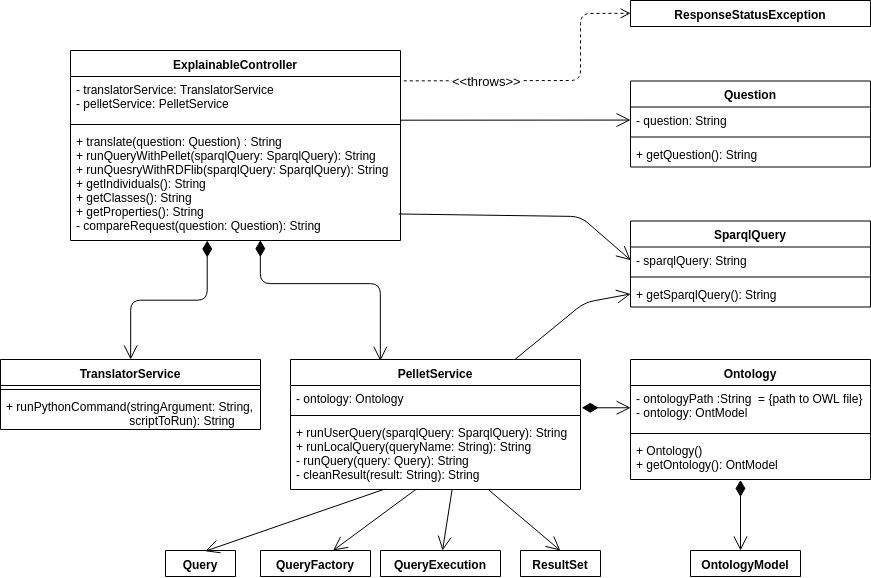
\includegraphics[width = 0.9\linewidth]{img/uml_server.png}
        \caption{Diagrama de clase a serverului {\it Reasoning Server}}
    \label{fig:uml_server}
\end{figure}

'In diagrama din figura ~\ref{fig:uml_server}, {\it ExplainableController} 'indepline'ste func'tia de controller al aplica'tiei. Este format din $translatorService$ 'si $pelletService$ a c'aror instan'te sunt aduse prin injectarea dependin'telor. Acestea au rolul de 'indeplinire a serviciilor, respectiv a logicii mai complexe pentru ob'tinerea r'aspunsurilor. $PelletService$ con'tine o instan't'a a ontologiei, $ontology$. Aceasta, la r\ia ndul ei este ob'tinut'a cu ajutorul fi'sierului OWL 'si a modelului pus la dispozi'tie de Pellet, $OntModel$. 'In plus fa't'a de $Ontology$, consider c'a clasele $Question$, $SparqlQuery$ sunt alte doua clase ce apar'tin modelului aplica'tiei, fiind utile 'in 'incapsularea datelor din request-uri.

$Query$ 'si $QueryFactory$ abstractizeaz'a o interogare 'in forma SPARQL care urmeaz'a a fi utilizat'a de Pellet pentru a ob'tine un r'aspuns de tipul $ResultSet$ prin intermediul $QueryExecution$. Acestea sunt clase care fac parte din libr'aria Pellet 'si nu le vom detalia.

Metoda $translate$ este apelat'a prin intermediul endpoint-ului {\it /translateQuery} 'si con'tinutul datelor transmise este un obiect din clasa $Question$, fiind o abstractizare a 'intreb'arii utilizatorului. Este utilizat'a pentru translatarea 'intreb'arii din limbaj natural 'in limbaj de interogare SPARQL.  Dac'a prin 'intrebare utiliztorul solicit'a compararea a doi algoritmi, se va utiliza metoda $compareRequest$ 'si se va returna o interogare SPARQL construit'a local. Altfel, aceasta apeleaz'a metoda $runPythonCommand$ din $TranslatorService$ 'si returneaz'a rezultatul dat de Quepy c'atre interfa'ta utilizator. Asem'an'ator, $runQueryWithRDFLib$ din controller este atins'a prin intermediul rutei {\it /runQueryWithRDFLib} 'si apeleaz'a aceea'si metod'a pentru rulare a comenzii , preciz\ia nd de data aceasta script-ul de ob'tinere a r'aspunsului cu RDFLib.

Metoda $runQueryWithPellet$ este folosit'a pentru ob'tinerea r'aspunsului la interogarea SPARQL print intermediul Pellet. Utilizeaz'a path-ul {\it /runQueryWithPellet} 'si va apela $runUserQuery$ din $PelletService$. 'In $runUserQuery$ se stabile'ste interogarea SPARQL a utilizatorului 'si se apeleaz'a $runUserQuery$. Prin $runQuery$, r'aspunsul este ob'tinut de la Pellet 'in format JSON utiliz'and clasele $QueryExecution$ 'si $ResultSet$, urm'and ca apoi acesta s'a fie cur'a'tat de prefixuri prin intermediul metodei $cleanResult$.

Metodele $getClasses$, $getIndividuals$ 'si $getProperties$ sunt accestate prin intermediul path-urilor $/classes$, $/individuals$ 'si respectiv $/properties$. Acestea au rolul de a ob'tine toate clasele ontolgiei, to'ti indivizii 'si toate propriet'a'tile. Utilizeaz'a metoda $runLocalQuery$ 'si interog'ari 'in limbaj SPARQL definite local. Pentru ob'tinerea r'aspunsului se folose'ste metoda $runQuery$, asem'an'ator cazului 'in care se utilizeaz'a interogarea utilizatorului.

Libr'aria Pellet reprezint'a suportul pentru modulul $Reasoning\ Server$ 'si realizeaz'a ob'tinerea r'aspunsului prin inferen'ta. Prin intermediul $ExplainableController$, utilizatorul are acces la translatarea din limbaj natural 'in limbaj de interogare SPARQL, c'at 'si la interogarea ontologiei prin Pellet sau prin RDFLib.

Sistemul este dezvoltat astfel 'inc\ia t sa permit'a 'intreruperea cursului aplica'tiei prin aruncarea excep'tiilor 'in cazul 'in care apar evenimente nedorite. Dac'a translatarea interog'arii din limbaj natural 'in limbaj de interogare SPARQL este defectuoas'a, sau dac'a interogarea SPARQL care se folose'ste pentru a chestiona ontologia prezint'a anomalii, din controller se arunc'a $ResponseStatusException$. Aceasta este o clas'a customizat'a pentru a 'ingloba statusul r'aspunsului, c'at 'si motivul 'intreruperii. 'Si 'in alte cazuri, cum ar fi 'in cazul c'ampurilor goale, se arunc'a aceast'a excep'tie, cu un mesaj corespunz'ator.

\section{Modulul de raspuns pe baza de graf}

Acest modul este destinat interog'arii ontologiei aflat'a 'in forma de graf RDF 'si folose'ste RDFLib pentru a pune 'in practic'a acest lucru. Utilizarea libr'ariei RDFLib este simpl'a, fiind necesar'a doar instalarea 'si importarea acesteia. Modulul 'in care am implementat interogarea ontologiei 'in format RDF este un script 'si vine 'in ajutor pentru momentele 'in care un query SPARQL are anumite particularit'a'ti semantice care nu sunt interpretate 'in acela'si mod de Pellet. 

\begin{figure}
\centering
\begin{lstlisting}[language=Python, basicstyle=\footnotesize,numbers=left, xleftmargin=.05\textwidth]
import json, re, sys
from rdflib import Graph

PREFIXES = ["http://www.semanticweb.org/machine-learning-ontology#",  
            "http://www.w3.org/2002/07/owl#"]


def to_json(query_response):
    list_result = []
    for row in query_response:
        dictionary_response = {}
        for i in range(len(row)):
            current_result = row[i]
            for prefix in PREFIXES:
                if prefix in row[i]:
                    current_result = re.sub(prefix, "", row[i])
            dictionary_response[row.labels.keys()[row.labels.values().index(i)]] \
                = current_result
            list_result.append(dictionary_response)

    json_result = json.dumps(list_result, sort_keys=False, indent=4)
    return json_result


query = sys.argv[1]
g = Graph()
g.parse(r'../ontologies/machine-learning-ontology.owl', format="xml")
query_response = g.query(query)
json_result = to_json(query_response)
print json_result

\end{lstlisting}
        \caption{Scriptul pentru interogare prin RDFLib}
      \label{fig:rdflib_script}
\end{figure}

'In figura ~\ref{fig:rdflib_script} primul pas 'in ob'tinerea unui r'aspuns la o interogare SPARQL este de a citi de la linia de comand'a interogarea SPARQL care a fost transmis'a, 'in cazul aplica'tiei noastre, de c'atre serviciul aferent din {\it Reanoning Service}. La liniile (26)-(25), se formeaz'a un graf 'si ontologia noastr'a este parsat'a si salvat'a sub forma de noduri de triple. 'In continuare, la linia (28), se afl'a r'aspunsul interog'arii SPARQL. R'aspunsul dat de RDFLib nu este compatibil cu formatul JSON 'si con'tine informa'tii despre prefixe care ar putea induce 'in eroare utilizatorul. Astfel c'a, am implementat func'tia $to\_json(query\_response)$, ilustrat'a 'in figura ~\ref{fig:rdflib_script} la liniile (8-22), pentru a transforma r'aspunsul in format JSON 'si a-l 'infrumuse'ta. 

'In final, raspunsul $json\_result$ va fi printat 'si preluat de c'atre server. Dup'a cum am mai amintit 'in acest capitol, r'aspunsul este trimis de c'atre server la interfa'a utilizator, unde va fi vizualizat de c'atre client.


\section{Modulul de translatare}
\subsection{Arhitectura 'si func'tionarea translatorului Quepy}

Modulul $Translator$ este construit 'in Python cu ajutorul framework-ului Quepy. Este destinat pars'arii 'si translat'arii 'intreb'arilor din limbaj natural 'in limbaj de interogare SPARQL. Aceste interog'ari SPARQL sunt utilizate pentru a interoga ontologia despre $machine-learning$. Modulul este generat automat de o comand'a quepy, iar 'in figura ~\ref{fig:quepy_files} se pot observa componentele necesare modulului $Translator$ de care facem uz 'in aceast'a aplica'tie. 
\begin{figure}
    \centering
    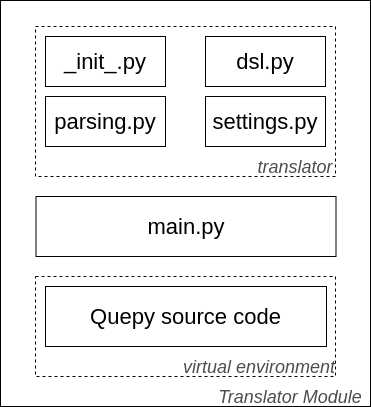
\includegraphics[width = 0.5\linewidth]{img/quepy_schema.png}
    \caption{Componentele modulului $Translator$}
    \label{fig:quepy_files}
\end{figure}

Fi'sierul $\_init\_.py$ constituie punctul de plecare al aplica'tiei, fi'sierul de ini'tializare. 'In acesta se import'a fi'sierul $parsing.py$, iar la instalarea aplica'tiei va fi citit prin intermediul $\_init\_.py$. 

Unul dintre cele mai importante fi'siere ale acestui modul este $parsing.py$. Acesta con'tine toate regulile de parsare ale aplica'tiei. 'In acest fi'sier sunt declarate toate 'intreb'arile permise de sitemul nostru, sub forma de patternuri. 'In sec'tiiunea ~\ref{sec:parse} vom detalia acest fi'sier, 'impreuna cu procedeul de dezvoltare.

Fi'sierul $settings.py$ presupune locul 'in care se declara toate prefix-urile necesare unei interog'ari SPARQL, cum ar fi 'in cazul nostru prefixul pentru ontologia noastr'a 'si altele. Tot 'in acest loc, se decide limbajul de interogare, care 'in modulul $Translator$ este SPARQL.

Limbajul specific al domeniului este definit in $dsl.py$, fi'sier 'in care am adaugat toate clasele ontologiei noastre, 'impreuna cu propriet'a'tile acestora. Modul de detaliere al ontologiei, exemple de clase din acest fi'sier 'si o descriere mai larga a acestuia sunt 'in sec'tiunea ~\ref{sec:dsl}. 

Fi'sierul $main.py$ con'tine logica de pornire a aplica'tiei. 'In acesta am apelat ini'tializarea translatorului, am citit 'intrebarea utilizatorului din argumentele liniei de comand'a 'si am solicitat transformarea acesteia 'in SPARQL. 
Datorit'a faptului c'a am modificat 'si unele elemente ale libr'ariei pentru a implementa operatorii logici, am ales reprezentarea acesteia 'in imagine, 'in mediu virtual creat la formarea aplica'tiei.

$Translatorul$ este unul dintre cele mai importante module ale sistemului nostru, efectu\ia nd transaltarea din limbaj natural 'in limbaj de interogare SPARQL. Dupa ce utilizatorul introduce o 'intrebare 'in limbaj natural 'si cere traducerea sa 'in SPARQL, modulul este ini'tializat. 'In acest pas, toate regulile definite de noi 'in fi'sierul $parsing.py$ sunt 'inregistrate spre a fi folosite. 
'Intrebarea utilizatorului este 'imp'ar'tit'a 'in cuvinte 'in func'tie de partea de vorbire pe care o reprezint'a. Se decide c'arei reguli se supune 'intrebarea adresat'a. Odat'a identificat'a regula, se folosesc clasele 'si regulile ontologiei definite 'in $dsl.py$ pentru a construi o interogare SPARQL restric'tionat'a de modul de interpretare decis de noi. 


\subsection{'Incorporarea elementelor ontologiei 'in Quepy}
\label{sec:dsl}

Pentru a putea construi interog'ari potrivite pentru o ontologie, modulul Quepy trebui customizat pentru a cunoa'ste clasele 'si propriet'a'tile din ontologie, c\ia t 'si alte reguli care sunt necesare a fi integrate 'in interog'ari. 'In fi'sierul $dsl.py$ am definit clasele asem'an'ator exemplului de cod ~\ref{lst:learning_meth_op}: 
\begin{lstlisting}[basicstyle=\footnotesize, language = Python, label = lst:learning_meth_op, caption = Clasa LearningMethod]
   class IsLearningMethod(FixedType):
    fixedtype = "ml:LearningMethod"

    def __init__(self, operator):
        super(IsLearningMethod, self).__init__(operator)
        self.fixedtype = operator + "ml:LearningMethod"

\end{lstlisting}

Acesta este un exemplu 'in care am 'incadrat 'si 'imbun'at'a'tirile aduse libr'ariei, 'si anume suportul pentru o operatorii logici. Propriet'a'tile sunt definite asem'an'ator cu exemplul de cod ~\ref{lst:learning_meth_rel}:

\begin{lstlisting}[basicstyle=\footnotesize, language = Python, label = lst:learning_meth_rel, caption = Proprietatea has-learning-method]
class HasLearningMethodReversed(FixedRelation):
    relation = "ml:has-learning-method"
    reverse = True

class NotHasLearningMethod(MinusFixedRelation):
    relation = "ml:has-learning-method"
    reverse = False

class HasLearningMethod(FixedRelation):
    relation = "ml:has-learning-method"
    reverse = False

\end{lstlisting}

'In acest exemplu am 'incadrat rela'tia invers'a, rela'tia implementat'a de mine pentru a sus'tine operatorul $MINUS$ cu func'tia de $not$, 'si rela'tia simpl'a.


\subsection{Parsarea 'intreb'arilor}
\label{sec:parse}

'In fisierul $parsing.py$ am definit toate regulile de parsare ale 'intreb'arilor, un num'ar total de 15 clase asociate ficare c\ia te unei 'intreb'ari. Acestea con'tin regulile de parsare, 'impreuna cu o metod'a $interpret$ care specific'a ordinea 'in care vor fi ad'augate elementele identificate 'in interogare.

Figura ~\ref{fig:r1} detaliaz'a regula pentru identificarea indivizilor clasei $Algorithm$. 'In aceast'a regul'a, $target$ func'tioneaz'a ca 'inlocuitor pentru conceptul c'aruia dorim s'a 'i afi'sam indivizii. Poate fi substantiv (NN), substantiv propriu (NNP) sau substantiv la plural (NNS). Variabila $optional\_opening$ este un 'inlocuitor pentru {\it"What are the"} sau {\it"Which are the"} 'si este op'tional'a, a'a cum este definit de comportamentul func'tiei $Question$. Prin $Lemma("be")$ 'in'telegem cuv\ia ntul de baz'a 'si inflexiunile sale, adic'a toate formele verbului $"to\ be"$.
Expresiile $regex1$ 'si $regex2$ sunt cuprinse 'in $regex$ 'si reprezint'a toate formele acceptate ale 'intreb'arii.

\begin{figure}[h]
\centering
\begin{lstlisting}[basicstyle=\footnotesize, numbers=left, xleftmargin=.05\textwidth]
target = Group (Pos("NN") | 
                Pos("NNP") | 
                Pos("NNS"), "target")
opt_opening = Question((Pos("WP") | 
                        Pos("WDT")) + 
                          Lemma("be") + 
                          Pos("DT"))
regex1 = optOpening + 
         Question(Lemma("individual") | 
                  Lemma("instance")) + 
                    Pos("IN") + target + 
                    Question(Pos("."))
regex2 = Question(Lemma("list") | 
                  Lemma("show") | 
                  Lemma("print")) + target +   
                  Question(Lemma("individual") |
                           Lemma("instance"))
regex = regex1 | regex2
  \end{lstlisting}
        \caption{Rule $R_1$ for listing individuals.}
      \label{fig:r1}
  \end{figure}
  
  \begin{example}[Aplicare $R_1$] 
  Fie 'intrebarea {\it What are the individuals of Algorithm?}
  Aceasta face match pe $regex1$ dup'a cum urmeaz'a:
  
   %\begin{table}[h]
%      \caption{regex and matching words}
 %     \centering
 %\vspace{0.3cm}
    \begin{center}
      \begin{tabular}{ll}
      regex part & word\\ \hline
      
  {\it Pos("WP")} & What\\
  {\it Lemma("be")} & are\\
  {\it Pos("DT")} & the\\
  {\it Lemma("individual")} & individuals\\
  {\it Pos("IN")} & of\\
  {\it target} & Algorithm\\
       \end{tabular}
       \end{center}
        \vspace{0.3cm}
   \end{example}

\subsection{'Imbun'at'a'tiri aduse libr'ariei Quepy}

'In limbajele de interogare exista necesitatea utiliz'arii operatorilor logici, c'at 'si a unui operator de selec'tie a datelor 'in func'tie de nume. SPARQL ofer'a suport pentru operatorii logici prin intermediul operatorului $FILTER$. Framework-ul de translatarea  'intreb'arilor din limbaj natural 'in limbaj de interogare SPARQL, Quepy, implementeaz'a o solu'tie pentru $FILTER$ numit'a $HasKeyword$ care nu este func'tional'a nici 'in Pellet, 'si nici 'in RDFLib. 

Astfel, din necesitatea de a avea un operator pentru extragerea selectiv'a a datelor am implementat $FILTER$. Pe baza operatorului $FILTER$ am implementat suport 'si pentru operatorii logici: $AND$, $OR$ 'si $NOT$, care este utilizat 'in SPARQL sub numele de $MINUS$. Operatorul $MINUS$ realiza'a negarea prin diferen'ta mul'timilor. To'ti ace'stia se dovedesc a fi extrem de necesari 'in dezvoltarea unor 'intreb'ari mult mai complexe 'si flexibile, cum ar fi:


  
  \begin{example} Utilitatea operatorilor implementa'ti 'in 'intreb'ari
  
 \begin{center}
      \begin{tabular}{ll}
      operator & 'intrebare\\ \hline
      
  {\it FILTER } & What are the learning methods of sarsa?\\
  {\it AND} & algorithm that solves classification problem \\
            & and has supervised learning method \\
            & and has feature complexInteractions \\
  {\it OR } & algorithm suitable for nonLinearModels or shortDocuments\\
  {\it MINUS} & algorithms that do not have supervised learning method\\
       \end{tabular}
       \end{center}
        \vspace{0.3cm}
   \end{example}

La baza operatorului $FILTER$ stau clasele $FixedInstance$ 'si $HasInstance$, imediat prezentate. Acestea sunt implementate pentru a oferi suport operatorului $FILTER$, 'impreun'a cu $AND$ 'si $OR$. Clasa $HasInstance$ extinde clasa $FixedInstance$ 'si defineste relatia "FILTER". Clasa $FixedInstance$ este asem'an'atoare clasei $FixedType$ din libr'aria Quepy. Aceasta este subclas'a a clasei $Expression$ din libr'arie 'si implementeaz'a adaugarea operatorului la rela'tie. 

\begin{lstlisting}[basicstyle=\footnotesize, language = Python]
class FixedInstance(Expression):
    relation = None

    def _init_(self, data, operator):
        super(FixedInstance, self)._init_()
        # ...
        self.relation = encoding_flexible_conversion(operator + self.relation)
        self.add_data(self.relation, data)
        
class HasInstance(FixedInstance):
    relation = u"FILTER"

    def _init_(self, data, operator):
        super(HasInstance, self)._init_(data, operator)

\end{lstlisting}

Pentru implementarea rela'tiei $MINUS$ am ad'augat clasa $MinusFixedRelation$ 'in fisierul $dsl.py$, implementat'a dupa modelul $FixedRelation$, proprietate a libr'ariei. $MinusFixedRelation$ extinde clasa $Expression$ din libr'aria Quepy.'In acceasta am ad'augat suport pentru implementarea operatorului $MINUS$, ad'augat la rela'tia pe care o neag'a. 

\begin{lstlisting}[basicstyle=\footnotesize, language = Python]
class MinusFixedRelation(Expression):
relation = None
reverse = False

def _init_(self, destination, reverse=None):
    if reverse is None:
        reverse = self.reverse
    super(MinusFixedRelation, self)._init_()
    # ...
    self.relation = "MINUS " + self.relation
    self.nodes = copy(destination.nodes)
    self.head = destination.head
    self.decapitate(self.relation, reverse)

\end{lstlisting}

Datorit'a faptului c'a operatorii noi $FILTER$, $AND\ FILTER$, $OR\ FILTER$ 'si $MINUS$ sunt operatori prefix, iar Quepy implementeaz'a original numai operatori infix, a fost necesar'a modificarea func'tiei de construc'tie a interog'arii SPARQL pentru a realiza construc'tia corect'a a interog'arii. Func'tia respectiv'a se nume'ste $expression\_to\_sparql$ 'si este g'asit'a 'in fi'sierul $sparql\_generation.py$, din libr'aria Quepy. Am extins aceast'a func'tie utiliz'and operatori condi'tionali $if$, ad'aug\ia nd logic'a pentru concatenarea constr\ia ngerilor multiple 'in FILTER.

\section{Modulul ontologiei}
Ontologia noastr'a reprezint'a nivelul de persisten't'a al aplica'tiei, sursa din care sunt extrase informa'tiile pentru r'aspunsul 'intreb'arilor. Aceasta sumarizeaz'a cuno'stin'te despre {\it machine learning} 'si este structurat'a 'in concepte, roluri 'si indivizi. 'In aceast'a sec'tiune, vom relata arhitectura ontologiei, c'at 'si ce con'tine aceasta 'si felul 'in care au fost selectate datele. 

Construc'tia unei ontologii complete pentru machine learning presupune nenum'arate dificult'a'ti de care suntem con'stien'ti. Astfel c'a, am dezvoltat un prototip pentru a ilustra func'tionalit'a'tile sitemului nostru. Am cuprins o vedere de ansamblu a domeniului, informa'tii care stau la baza acestuia si care sunt necesare pentru o baz'a solid'a. Ontologia prezentat'a formalizeaz'a cuno'stin'tele pentru 340 de indivizi, 56 de concepte si 9 roluri din domeniul reprezentat de machine learning.

\begin{figure}[ht]
    \centering
    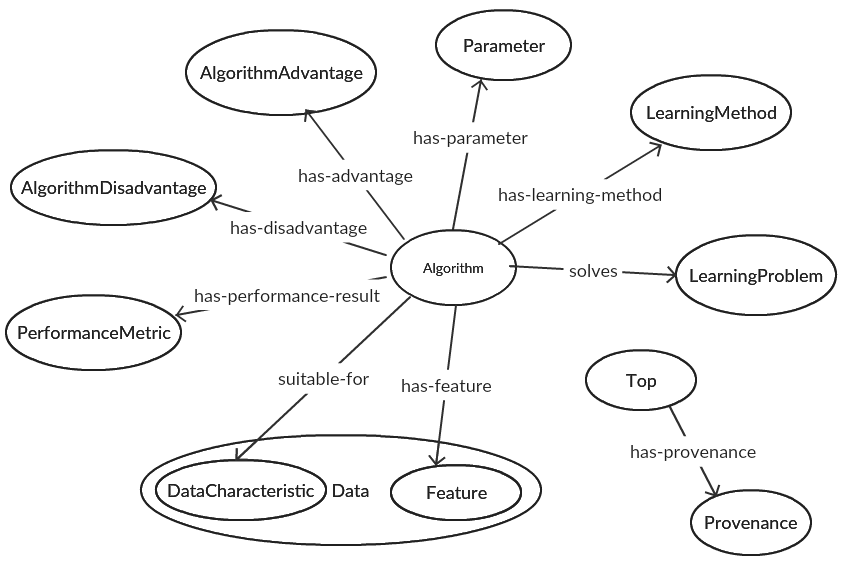
\includegraphics[width = 0.85 \linewidth]{img/ontologie_black.png}
        \caption{Vedere de ansamblu asupra ontologiei pentru machine learning: conceptul {\it Algorithm} 'si rolurile sale c'atre alte concepte.}
    \label{fig:onto}
\end{figure}

O vedere schematic'a asupra ontologiei apare 'in ~\ref{fig:onto}. 'In aceasta se pot observa rolurile care leag'a conceptul ML {\it Algorithm} de celelalte concepte din ontologie. Sunt expuse doar conceptele din primul nivel, excep'tie f'ac\i and clasa {\it Data} care este prezentat'a 'impreun'a cu cele dou'a subclase ale sale: {\it DataCharacteristic} 'si {\it Feature}. Imaginea eviden'tiaz'a datele con'tinute de ontologie: algoritmi, parametrii acestora, metode de 'inv'a'tare, problema de 'inv'a'tare pe care o rezolv'a, metrici de performan't'a, caracteristicile datelor 'si features, avantaje 'si dezavantaje, c\i at 'si informa'tii despre provenien'ta acestora.

\begin{figure}[h!]
    \centering
    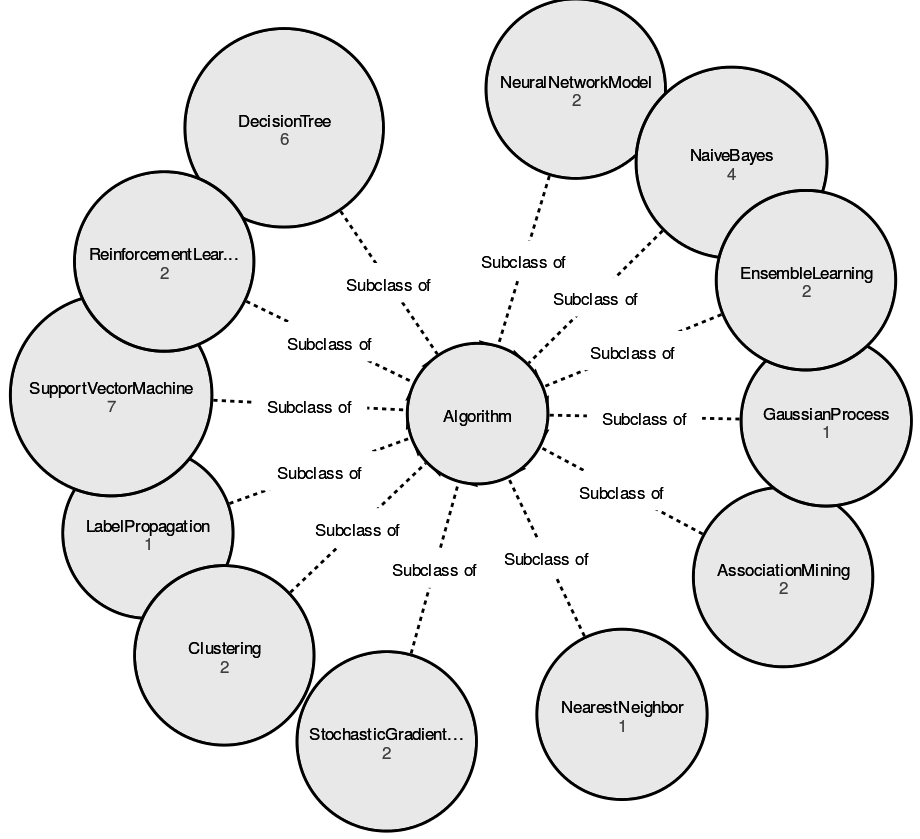
\includegraphics[width = 0.75 \linewidth]{img/algorithm_subclasses.png}
        \caption{Clasa {\it Algorithm}: diferiti algoritmi pentru ML}
    \label{fig:alg_sucls}
\end{figure}

Conceptul {\it Algorithm} este divizat 'in mai multe subconcepte care reprezint'a familii diferite de algoritmi, ce pot fi v'azute 'in Fig.~\ref{fig:alg_sucls}. Aduce 'impreun'a algoritmi care au metode de 'inv'a'tare supervizat'a, nesupervizat'a (cum ar fi clustering sau asociere), semi-supervizat'a 'si reinforcement. Cuprinde diferite varia'tii de algoritmi care sunt structura'ti 'in sublcase 'in func'tie de familia din care apar'tin: $DecisionTree$, $NeuralNetworkModel$, $NaiveBayes$, $SupportVectorMachine$, $LabelPropagation$ etc.

Similar conceptului de {\it Algorithm}, 'si parametrii sunt grupa'ti 'in clasa {\it Parameter} 'in func'tie de algoritmii c'arora le sunt asocia'ti. Figurile ~\ref{fig:subc_1} si ~\ref{fig:subc_2} ilustreaz'a acest fapt. Am ales divizarea parametrilor mai 'int\ia i 'in func'tie de familia de care apar'tin. Dac'a algoritmii din aceea'si familie nu folosesc aceia'si parametrii, am 'imp'ar'tit mai departe ace'sti parametrii 'in func'tie de indivizii c'arora le sunt asocia'ti. Parametrii compu'si apar'tin fiecare clasei c'areia 'ii descrie. 

\begin{figure}
    \centering
    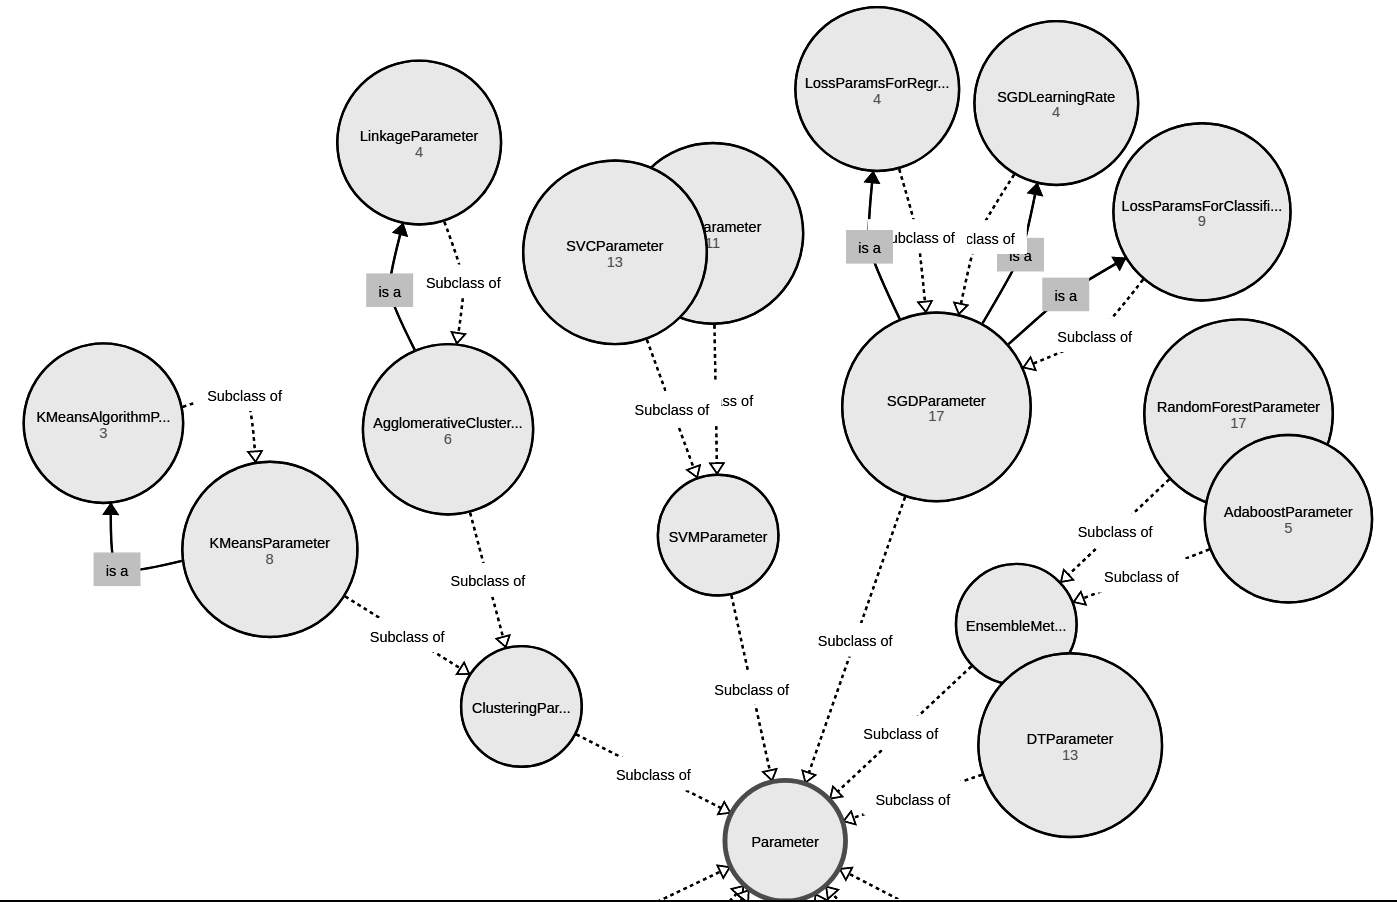
\includegraphics[width = 0.9 \linewidth]{img/properties_subcls_2.png}
        \caption{Prima parte a subconceptelor clasei $Parameter$}
    \label{fig:subc_1}
\end{figure}

\begin{figure}
    \centering
    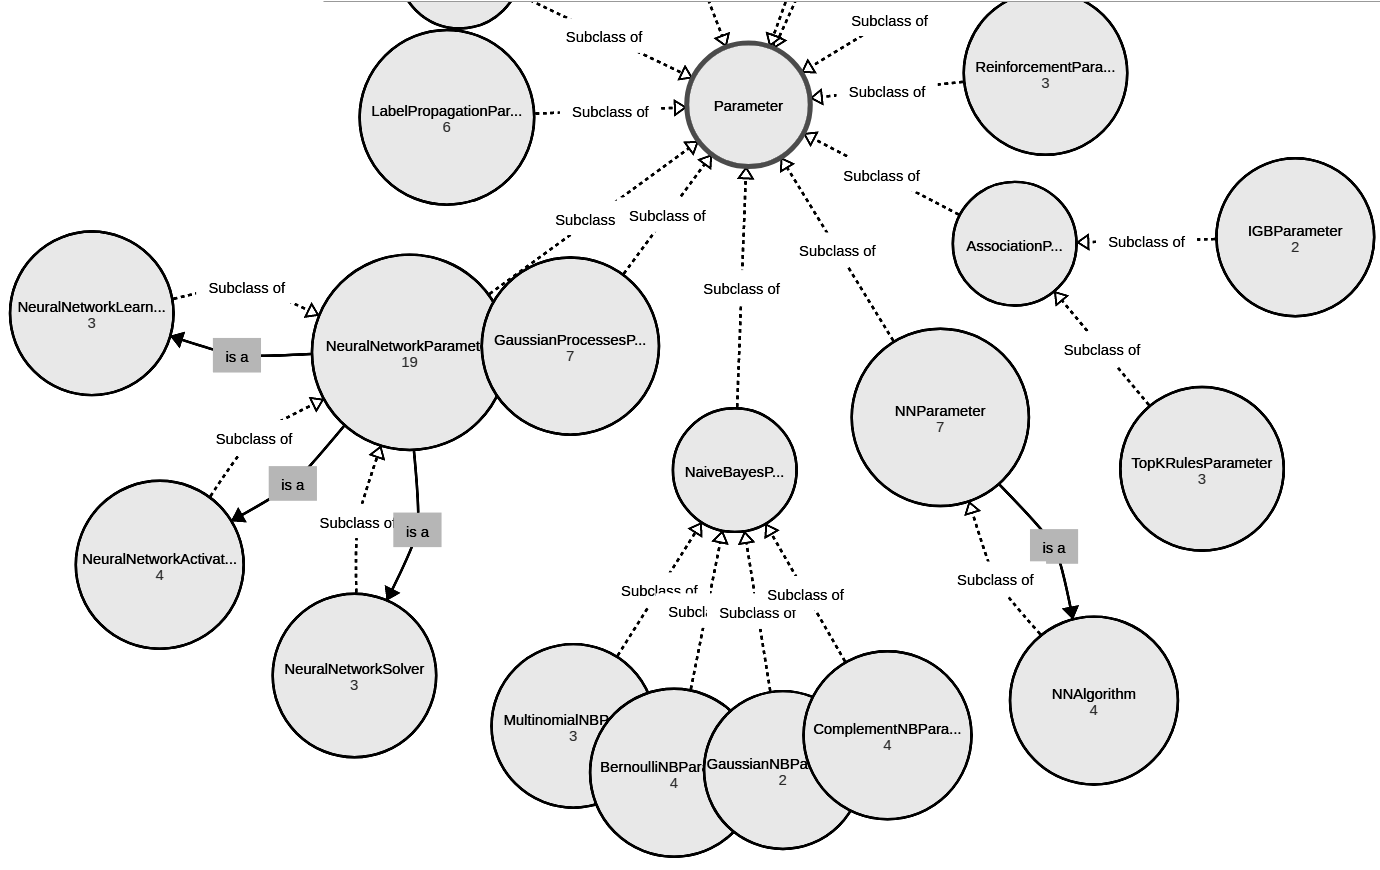
\includegraphics[width = 0.9 \linewidth]{img/properties_subcls_1.png}
        \caption{A doua parte a subconceptelor clasei $Parameter$}
    \label{fig:subc_2}
\end{figure}

Pentru popularea ontologiei ne-am bazat pe diferite tool-uri disponibile pentru ML. Pentru algoritmi pentru clustering, 'inv'a'tare semi-supervizat'a 'si superviza'ta, sursa principal'a de informa'tie este SciKit\footnote{https://scikit-learn.org/stable/}. Pentru association mining, am utilizat spmf\footnote{http://www.philippe-fournier-viger.com/spmf}. Datele despre reinforcement provin de la UNSW Sydney\footnote{https://www.cse.unsw.edu.au/~cs9417ml/RL1/algorithms.html}. 
%Being implemented taking into account good practices, our machine learning ontology can be further extended.


Ontologia a fost populat'a utiliz\ia nd Protege, acesta fiind o unealt'a automat'a pentru construirea ontologiilor. Permite ad'augarea conceptelor, a propriet'a'tilor 'si a indivizilor 'si genereaz'a un fi'sier 'in formatul dorit, OWL. Prezent'am in continuare exemple de implementare.

Proprietatea $has-learning-method$ prezint'a domeniul $Algorithm$ 'si codomeniul (range) $LearningMethod$ 'si este definit'a astfel:
\begin{lstlisting}[basicstyle=\footnotesize]

<owl:ObjectProperty rdf:about="http://www.semanticweb.org/machine-learning-ontology
                                #has-learning-method">
    <rdfs:domain rdf:resource="http://www.semanticweb.org/machine-learning-ontology
                                #Algorithm"/>
    <rdfs:range rdf:resource="http://www.semanticweb.org/machine-learning-ontology
                                #LearningMethod"/>
</owl:ObjectProperty>
\end{lstlisting}


 Clasa $Algorithm$ este definit'a astfel 'in fi'sierul OWL:
\begin{lstlisting}[basicstyle=\footnotesize]
    <owl:Class rdf:about="http://www.semanticweb.org/machine-learning-ontology
                        #Algorithm"/>
 \end{lstlisting}   

O subclas'a a clasei $Algorithm$, $EnsembleMethod$, con'tine 'in defini'tia sa o leg'atur'a c'atre superclas'a si un comentariu:
\begin{lstlisting}[basicstyle=\footnotesize]
    <owl:Class rdf:about="http://www.semanticweb.org/machine-learning-ontology
                        #EnsembleLearning">
        <rdfs:subClassOf rdf:resource="http://www.semanticweb.org
                             /machine-learning-ontology #Algorithm"/>
        <rdfs:comment>
            The goal of ensemble methods is to combine the predictions
            of several base estimators built with a given learning algorithm in
            order to improve generalizability / robustness over a single estimator.
        </rdfs:comment>
    </owl:Class>
    
\end{lstlisting}
Individul $classification$ face parte din clasa $LearningProblem$ 'si este definit astfel: 

\begin{lstlisting}[basicstyle=\footnotesize]
    <owl:NamedIndividual rdf:about="http://www.semanticweb.org
                        /machine-learning-ontology#classification">
        <rdf:type rdf:resource="http://www.semanticweb.org
                        /machine-learning-ontology#LearningProblem"/>
    </owl:NamedIndividual>
    
\end{lstlisting}


'In tabelul ~\ref{table:individuals_table} prezent'am pentru un exemplu de algoritm, $decisionTreeClassifier$, propriet'a'tile 'si indivizii din codomeniul acestora. 

\begin{table}[ht]
\caption{Indivizi ai ontologiei}
\centering                          % tabel centrat 
\begin{tabular}{|c|c|c|c|}          % 4 coloane centrate 
\hline\hline                        % linie orizontala dubla
Proprietate& Indivizi & Clasa indivizilor \\ [0.5ex]   % inserare tabel
%heading
\hline                              % linie orizontal simpla
solves & classification & LearningProblem  \\               % corpul tabelului 
has-learning-method & supervised
& LearningMethod  \\[1ex]           % [1ex] adds vertical space
has-parameter &  \begin{tabular}{@{}c@{}} maxFeature, presort \\ max\_depth, class\_weight\end{tabular} & DTParameter \\[1ex]

suitable-for & nonLinearModels & DataCharacteristic \\[1ex]

has-feature-characteritic & complexInteractions & Feature \\[1ex]

has-advantage & whiteBox, handlesColinearity & AlgorithmAdvantage\\[1ex] 
has-disadvantage & proneToOutliers, proneToOverfitting & AlgorithmDisadvantage \\[1ex]

has-provenance & scikitSupervised & Provenance \\[1ex]

\hline                              
\end{tabular}
  % titlul tabelului
\label{table:individuals_table}                % \label{table:nonlin} introduce eticheta folosita pentru referirea tabelului in text; referirea in text se va face cu \ref{table:nonlin}
\end{table}

'In acest tabel am inserat numai o parte din propriet'a'tile algoritmului $decisionTree$, acestea fiind multe la num'ar. 'In acest fel, am detaliat 'in ontologie o mare majoritate a algoritmilor insera'ti. 


\section{Analiza arhitecturilor echivalente}

Arhitectura propus'a 'si implementat'a reprezint'a numai o solu'tie de rezolvare a problemei agentului explicativ 'in domeniul machine-learning. Are numeroase avantaje, cum ar fi: centralizarea tuturor apelurilor la un singur server, aspect de arhitectur'a pe niveluri 'si u'surin'ta de implementare. Un dezavantaj major al acesteia este acela c'a modulul $Reasoning\ Server$ fun'ctioneaz'a ca un intermediar 'intre $Tranlator$ 'si ontologie. 

'In figura ~\ref{fig:alternative_arh} se prezint'a o solu'tie alternativ'a care 'inl'atur'a dezavantajul men'tionat. Noua structur'a este modular'a 'si propune existen'ta a doua servere: $Reasoning\ Server$ 'si $Translator\ Server$.


\begin{figure}
    \centering
    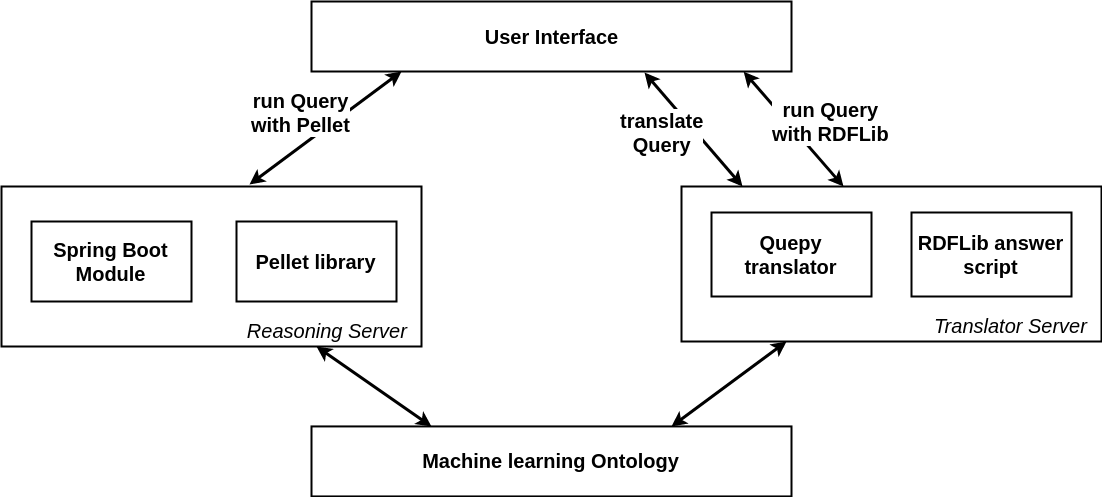
\includegraphics[width = 0.85 \linewidth]{img/arhitectura_alternativa.png}
        \caption{Arhitectur'a alternativ'a a aplica'tiei}
    \label{fig:alternative_arh}
\end{figure}

'In acest caz, $Reasoning\ Server$ va fi responsabil numai pentru request-urile care necesit'a utilizarea libr'ariei Pellet: interogarea ontologiei cu ajutorul Pellet, ob'tinerea claselor, a instan'telor 'si a propriet'a'tilor. $Translator\ Server$ devine responsabil pentru translatarea intreb'arilor din limbaj natural 'in limbaj de interogare SPARQL 'si pentru interogarea ontologiei folosind libr'aria RDFLib.

Arhitectura alternativ'a propus'a permite utilizarea modulului $Translator\ Service$ mult mai direct, f'ar'a 'int\ia rzieri. De'si pare o solu'tie mai potrivit'a pentru sistem, aceasta este dificil de implementat. Am 'incercat punerea 'in practic'a a acesteia 'inainte de varinta final'a din figura ~\ref{fig:arch}, dar am 'intampinat impedimente tehnice ale realiz'arii modulului $Translator$ sub form'a de server.



\section{Scenariu de utilizare}

'In figura ~\ref{fig:usecases} sunt prezentate func'tiile ce pot fi realizate din interfa't'a de c'atre utilizator. Acesta are posibilitatea de a scrie 'intrebarea, 'si, dup'a aceea, de a o translata 'in limbaj de interogare SPARQL. Utilizatorii mai avansa'ti pot edita interogarea SPARQL. Dup'a ace'sti pa'si, utilizatorul poate interoga ontologia utiliz'and Pellet sau RDFLib.  R'aspunsul acestor ac'tiuni poate fi vizualizat. 'In fereastra alternativ'a, utilizatorul poate solicita s'a vizualizeze toate clasele ontologiei, toate rolurile 'si to'ti indivizii.


\begin{figure}
    \centering
    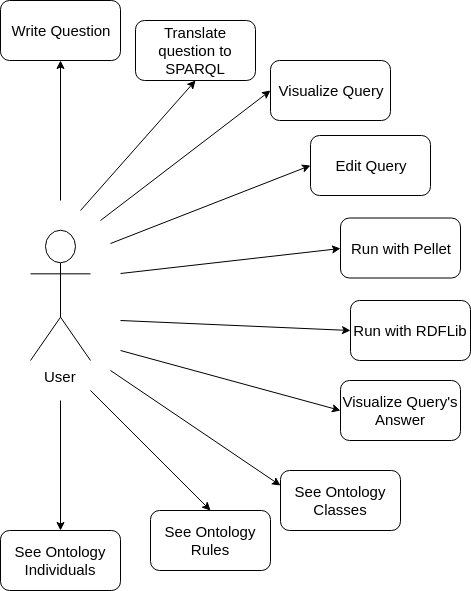
\includegraphics[width = 0.55 \linewidth]{img/use_case.png}
        \caption{Diagrama cazurilor de utilizare}
    \label{fig:usecases}
\end{figure}

'In continuare, vom ilustra capabilit'a'tile sistemului 'intr-un caz de utilizare.

Vom considera c'a utilizatorul ca'a utilizatorul introduce urm'atoarea 'intrebare:

\begin{center}
{\it $Q_1$: Which are the instances of algorithms?}
\end{center}

'Intrebarea poate fi formulat'a de asemenea ca {\it"individuals of Algorithm"},
       {\it "print Algorithm instances"},
       {\it "show Algorithms individuals"},
        {\it"list Algorithm"} 'si va fi interpretat'a 'si procesat'a 'in acela'si fel.
        
Cuv\ia ntul $individual$ poate fi 'inlocuit cu $instance$, dar poate de asemenea s'a 'si lipseasc'a. Dat fiind faptul c'a pluralul unui concept poate fi utilizat 'in mod obi'snuit, am considerat 'si acest caz.
Bazat pe regula Quepy $R_1$ (formalizat'a 'in sectiunea ~\ref{sec:parse}) interogarea SPARQL corespunz'atoare pentru $Q_1$ apare 'in Listing~\ref{lst:sparql:q1}.

%PREFIX owl:<http://www.w3.org/2002/07/owl#>
%PREFIX rdfs:<http://www.w3.org/2000/01/rdf-schema#>
\begin{figure}
\begin{footnotesize}
\begin{lstlisting}[captionpos=b, caption=Formalizarea SPARQL a interog'arii $Q_1$., label=lst:sparql:q1,
   basicstyle=\ttfamily,frame=single]
PREFIX rdf:<http://www.w3.org/1999/02/
           22-rdf-syntax-ns#>
PREFIX foaf:<http://xmlns.com/foaf/0.1/>
PREFIX skos:<http://www.w3.org/2004/02/skos/core#>
PREFIX quepy:<http://www.machinalis.com/quepy#>
PREFIX ml:<http://www.semanticweb.org/
           machine-learning-ontology#>

SELECT DISTINCT ?x0 WHERE {
  ?x0 rdf:type ml:Algorithm.
}
\end{lstlisting}
\end{footnotesize}
\end{figure}

Folosind Pellet, r'aspunsul $a_1$ este

\begin{center}
\begin{lstlisting}[basicstyle=\footnotesize]
{"head": { "vars": [ "x0" ]} ,
  "results": {
    "bindings": [
      {"x0":{"value":"gaussianProcessRegressor"}},
      {"x0":{"value":"oneClassSVM" }} 
      ...
      {"x0": {"value":"decisionTreeClassifier"}}]}}
\end{lstlisting}
\end{center}
unde variabilae $?x0$ 'inlocuie'ste instan'tele conceptului {\it Algorithm}. 

R'aspunsul este ob'tinut pe baza urm'atoarelor axiome generale de incluziune 'in logic'a descriptiv'a:

\vspace*{0.3cm}
\begin{tabular}{ll}
1. & $GaussianProcess  \sqsubseteq Algorithm$\\
2. & $SupportVectorMachine  \sqsubseteq Algorithm$\\
3. & $DecisionTree  \sqsubseteq Algorithm$\\
4. & $gaussianProcessRegressor: GaussianProcess$\\
5. & $oneClassSVM: SupportVectorMachine$\\
6. & $decisionTreeClassifier: DecisionTree$\\
\end{tabular}
\vspace*{0.3cm}

Din axiomele (1) 'si (2) Pellet deduce c'a $GaussianProcess$, $DecisionTree$ 'si $SupportVectorMachine$ sunt subconcepte ale clasei $Algorithm$. Fiind date axiomele (4), (5) 'si (6), Pellet infer'a c'a $gaussianProcessRegressor$, $oneCLassSVM$ 'si $decisionTreeClassifier$ sunt de asemenea indivizi ai conceptului $Algorithm$. 

Diferit, utiliz\ia nd RDFLib, r'aspunsul este o lista goal'a deoarece RDFLib nu poate s'a fac'a reasoning pe axiomele date 'si nu poate deduce c'a $gaussianProcessRegressor$, $oneCLassSVM$ 'si $decisionTreeClassifier$ sunt indivizi ai clasei $Algorithm$. 
'In acest caz, dac'a am fi dorit indivizii clasei $DecisionTree$ atunci RDFLib ar fi putut r'aspunde corect cu o list'a de indivizi.

De exemplu, fiind dat'a interogarea din Listing~\ref{lst:sparql:dt} 'in care cerem instan'tele conceptului $DecisionTree$:


\begin{figure}[h]
\begin{footnotesize}
\begin{lstlisting}[captionpos=b, caption=Interogare SPARQL pentru ob'tinerea indivizilor clasei $DecisionTree$, label=lst:sparql:dt,
   basicstyle=\ttfamily,frame=single]
SELECT DISTINCT ?x0 WHERE {
  ?x0 rdf:type ml:DecisionTree.}
\end{lstlisting}
\end{footnotesize}
\end{figure}

R'aspunsul $a_2$ ob'tinut cu RDFLib este:

\begin{center}
\begin{lstlisting}[basicstyle=\footnotesize]
    [{ "x0": "decisionTreeRegressor"}, 
    ...
    {"x0": "decisionTreeClassifier"}, 
    {"x0": "id3"}]
\end{lstlisting}
\end{center}
%%%%%%%%%%%%%%%%%%%%%%%%%%%%%%%%%%%%%%%%%%%%%%%%%%%%%%%%%%%%%%%%%%%%%%%%%%%
\chapter{Testare 'si Validare}

\subsection{Performan't'a}

Am evaluat aplica'tia utiliz\ia nd un set de 10 'intreb'ari pe care le-am rulat de 100 de ori. Am calculat media ob'tinerii unei interog'ari SPARQL 'si um'arul de constr'angeri pe care 'il are aceasta, num'arul de indivizi din r'aspunsul dat de Pellet 'si timpul afl'arii acestui r'aspuns, num'arul de instan'te con'tinute de r'aspunsul dat de RDFLib 'si timpul 'in care acesta a fost ob'tinut. 

Am utilizat urm'atoarele 'intreb'ari, unde $TQ$ refer'a o 'intrebare de test (test question):
\newline

\begin{small}
\begin{tabular}{ll}
$TQ_1$ & list Algorithm individuals\\
$TQ_2$ & list DecisionTree individuals\\
$TQ_3$ & sarsa learning methods\\
$TQ_4$ & What are the advantages of kMeans?\\
$TQ_5$ & show details of identity\\
$TQ_6$ & Data subclass\\
$TQ_7$ & class of mlpRegressor\\
$TQ_8$ & algorithm that solves classification problem and has\\
 & supervised learning method and has feature \\
 & complexInteractions \\
$TQ_9$ & algorithms that do not have supervised learning  \\
& method \\
$TQ_{10}$ & algorithm suitable for nonLinearModels \\
& or shortDocuments\\
\end{tabular}
\end{small}

'In tabelul ~\ref{table:performance} pot fi observate rezultatele acestei analize. Datorit'a arhitecturii sistemului, timpul ob'tinerii r'aspunsurilor de la modulul $Translator$ este 'int\ia rziat cu aproximativ 1 secunda. 'In schimb, libr'aria Pellet extrage r'aspunsul 'intr-un timp foarte bun. De'si acesta a fost scopul acestei analize, nu am puut constanta o leg'atur'a clar'a 'intre num'arul de r'aspunsuri 'si timpul necesar execu'tiei 'intreb'arilor.
\begin{table}
\caption{Performan'ta sistemului}
\centering                          % tabel centrat 
\begin{tabular}{|c|c|c|c|c|c|c|}          % 4 coloane centrate 
\hline\hline                        % linie orizontala dubla
TQ &  Constr\ia ngeri  & Quepy  & Nr. de rezultate & Pellet  & Nr. de rezultate  & RDFLib \\ [0.5ex]   % inserare tabel
& SPARQL & time(ms) & Pellet & Time(ms) & RDFLib & time(ms)\\ [0.5ex]
%heading
\hline                              % linie orizontal simpla
$TQ_1$ & 1 & 1930 & 32 & 7  & 0 & 1902 \\[1ex]
$TQ_2$ & 1 & 1719 & 6  & 5 & 6 & 1691 \\[1ex]
$TQ_3$ & 3 & 1852 & 1  & 5 & 0 & 1782 \\[1ex]
$TQ_4$ & 3 & 1828 & 3  & 5 & 0 & 1899 \\[1ex]
$TQ_5$ & 3 & 1715 & 1  & 4 & 1 & 1657 \\[1ex]
$TQ_6$ & 2 & 1867 & 4  & 6 & 2 & 1672 \\[1ex]
$TQ_7$ & 2 & 1723 & 3  & 6 & 2 & 1667 \\[1ex]
$TQ_8$ & 8 & 1915 & 1  & 11 & 0 & 1786 \\[1ex]
$TQ_9$ & 3 & 1830 & 13  & 4 & 0 & 1774 \\[1ex]
$TQ_10$ & 6 & 2057 & 4 & 8 & 0 & 2083 \\[1ex]

\hline                              
\end{tabular}
  % titlul tabelului
\label{table:performance}                % \label{table:nonlin} introduce eticheta folosita pentru referirea tabelului in text; referirea in text se va face cu \ref{table:nonlin}
\end{table}

'In urma unei analize mai profunde 'si separate a $Translatorului$ am ob'tinut rezultatele din tabelul ~\ref{table:performance_tr}. 
\begin{table}
\caption{Performan'ta modulului $Translator$}
\centering                          % tabel centrat 
\begin{tabular}{|c|c|c|c|c|c|c|}          % 4 coloane centrate 
\hline\hline                        % linie orizontala dubla
TQ &  Constr\ia ngeri  & Quepy  & Nr. de rezultate  & RDFLib \\ [0.5ex]   % inserare tabel
& SPARQL & time(ms)  & RDFLib & time(ms)\\ [0.5ex]
%heading
\hline                              % linie orizontal simpla
$TQ_1$ & 1 & 23  & 0 & 23 \\[1ex]
$TQ_2$ & 1 & 3 & 6 & 8 \\[1ex]
$TQ_3$ & 3 & 2 & 0 & 19 \\[1ex]
$TQ_4$ & 3 & 1  & 0 & 19 \\[1ex]
$TQ_5$ & 3 & 3  & 1 & 19 \\[1ex]
$TQ_6$ & 2 & 3  & 2 & 17 \\[1ex]
$TQ_7$ & 2 & 3  & 2 & 17 \\[1ex]
$TQ_8$ & 8 & 5  & 0 & 41 \\[1ex]
$TQ_9$ & 3 & 4  & 0 & 24 \\[1ex]
$TQ_10$ & 6 & 2 & 0 & 32 \\[1ex]

\hline                              
\end{tabular}
  % titlul tabelului
\label{table:performance_tr}                % \label{table:nonlin} introduce eticheta folosita pentru referirea tabelului in text; referirea in text se va face cu \ref{table:nonlin}
\end{table}


Acestea de confirm'a faptul c'a transmisia datelor dintre $Translator$ 'si $Reasoning\ Service$ dureaz'a mult, dar ne arat'a 'sii o leg'atur'a 'intre numarul de rezultate ob'tinute de RDFLib 'si timpul de execu'tie pentru ob'tinerea acestora. Se poate observa c'a timpul scade odat'a cu cre'sterea num'arului de rezultate.
%%%%%%%%%%%%%%%%%%%%%%%%%%%%%%%%%%%%%%%%%%%%%%%%%%%%%%%%%%%%%%%%%%%%%%%%%%%
\chapter{Manual de Instalare 'si Utilizare}

\section{Instalarea sistemului}
\section{Manual de utilizare}



%%%%%%%%%%%%%%%%%%%%%%%%%%%%%%%%%%%%%%%%%%%%%%%%%%%%%%%%%%%%%%%%%%%%%%%%%%
\chapter{Concluzii}

\section{Contribu'tii 'si realiz'ari}
\section{Dezvolt'ari ulterioare}


%\addcontentsline {toc}{chapter}{Bibliography} 
\bibliographystyle{IEEEtran} 
\bibliography{thesis}%same file name as for .bib

\appendix
\chapter{Sec'tiuni relevante din cod}

\begin{verbatim}
 /** Maps are easy to use in Scala. */
object Maps {
  val colors = Map("red" -> 0xFF0000,
                   "turquoise" -> 0x00FFFF,
                   "black" -> 0x000000,
                   "orange" -> 0xFF8040,
                   "brown" -> 0x804000)
  def main(args: Array[String]) {
    for (name <- args) println(
      colors.get(name) match {
        case Some(code) =>
          name + " has code: " + code
        case None =>
          "Unknown color: " + name
      }
    )
  }
}
\end{verbatim}

\chapter{Alte informa'tii relevante (demonstra'tii etc.)}

\textcolor{green}{LISTA DE INTREBARI PERMISE}

\chapter{Lucr'ari publicate (dac'a exist'a)}

Agentul explicabil pentru 'inv'a'tare automat'a descris 'in aceast'a lucrare a fost prezentat 'si 'in articolul "Towards Explainable Machine Learning Using  Natural Language Processing and Ontologies". Articolul este trimis la "IEEE 15th International Conference on
Intelligent Computer Communication and Processing (ICCP 2019)" 'si se afl'a in curs de verificare. Cu o variant'a restr\ia ns'a a acestuia am participat la "Conferin'ta 'Stiin'tific'a a Studen'tilor Sec'tiilor de Calculatoare 2019".
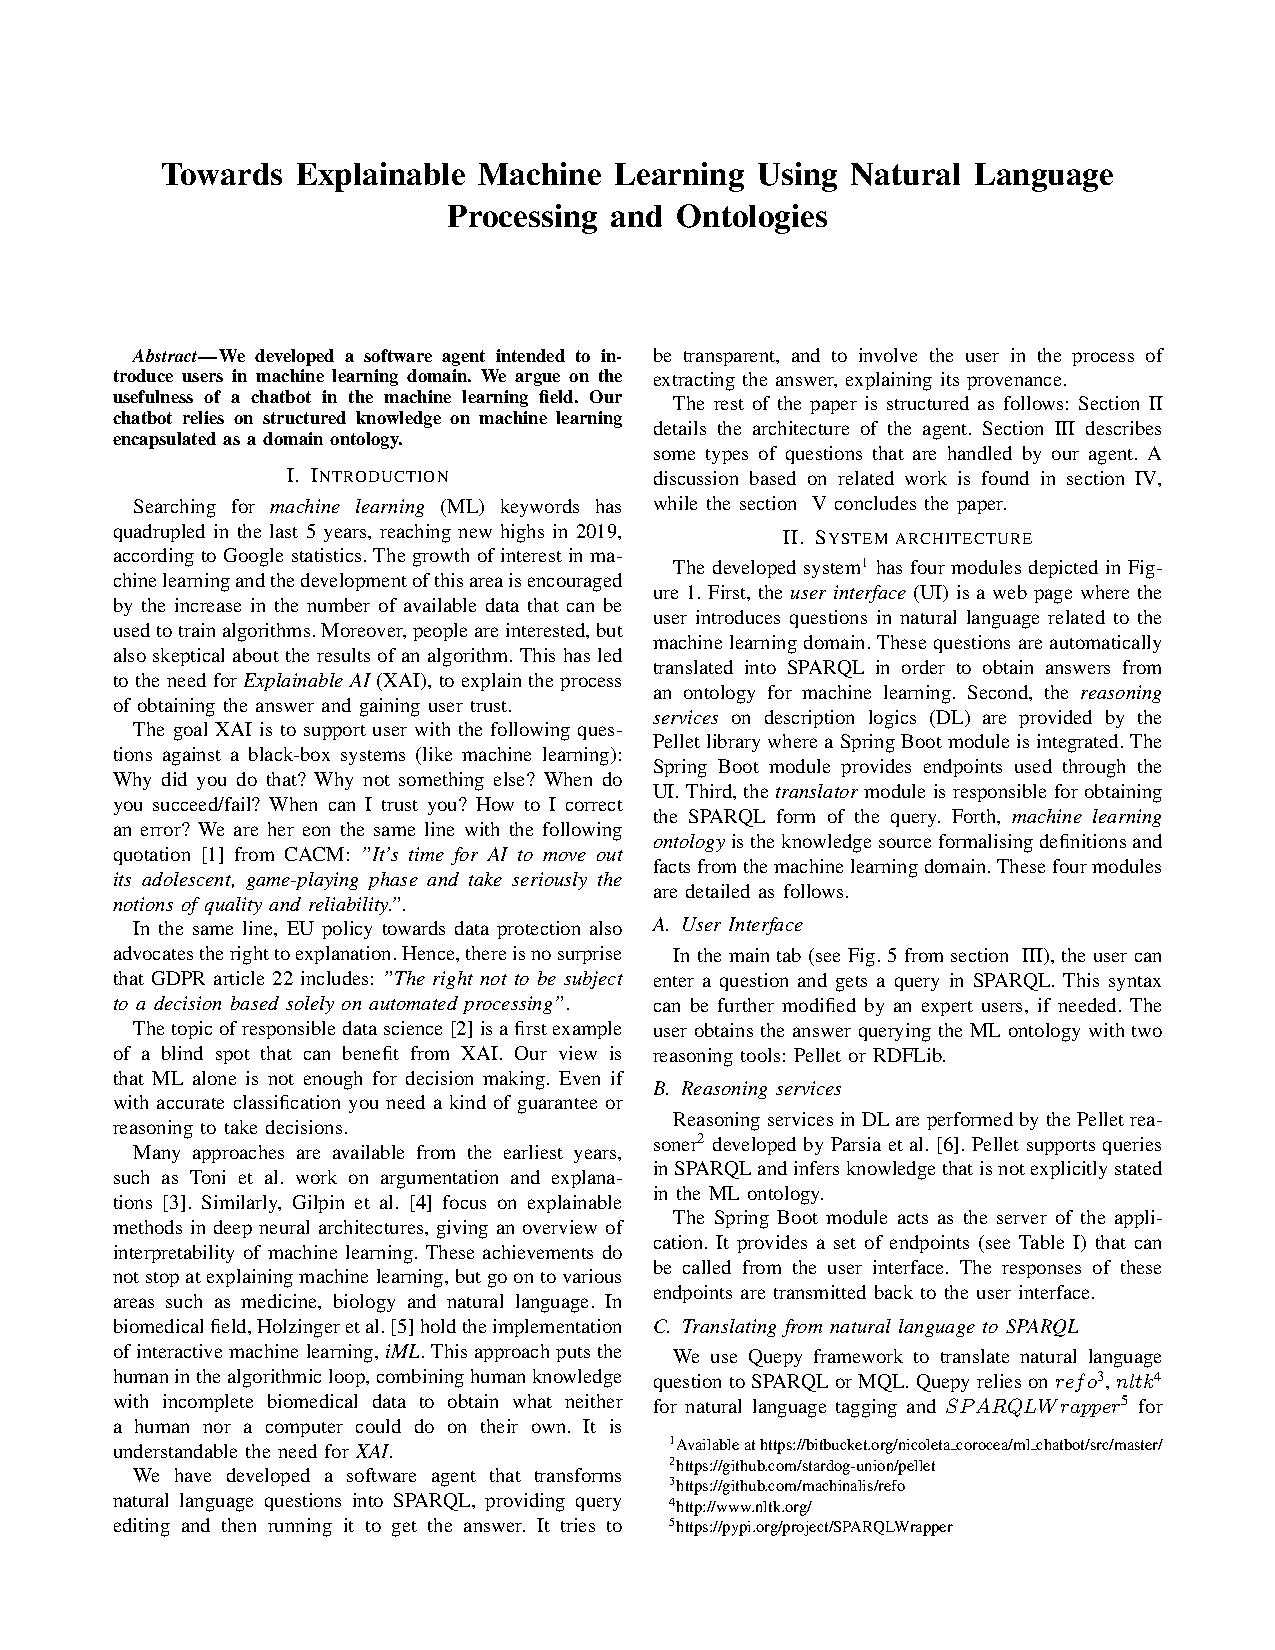
\includepdf[pages=-,pagecommand={},width=\textwidth]{articol_extins.pdf}


\textcolor{green}{lista completa cu intrebarile permise}

\end{document}
